\documentclass[spanish]{scrartcl}
\usepackage[spanish]{babel}
\selectlanguage{spanish}
\usepackage[utf8]{inputenc}
\usepackage{listings}
\usepackage{amsmath}
\usepackage[backend=biber]{biblatex}
\usepackage{graphicx}
\usepackage[usenames,dvipsnames]{color} % Required for specifying custom colors and referring to colors by name
\usepackage[colorlinks=true,linkcolor=blue,citecolor=blue,urlcolor=blue]{hyperref}

\lstset{language=Python, frame=single}
\let\endtitlepage\relax
\renewcommand{\and}{\vspace{1cm}}
\subtitle{Métodos Numéricos Avanzados}
\title{Speech Compression}
\author{
Juan Pablo Orsay - 49373 \\
Horacio Miguel Gomez - 50825 \\
Sebastián Andrés Maio - 50386 \\
Federico Bond - 52247 \\
Braulio Sespede - 51074
}
\date{Noviembre 2016}
\bibliography{informe}
\definecolor{DarkGreen}{rgb}{0.0,0.4,0.0} % Comment color
\definecolor{highlight}{RGB}{255,251,204} % Code highlight color

\lstdefinestyle{Style1}{ % Define a style for your code snippet, multiple definitions can be made if, for example, you wish to insert multiple code snippets using different programming languages into one document
language=Python, % Detects keywords, comments, strings, functions, etc for the language specified
basicstyle=\footnotesize\ttfamily, % The default font size and style of the code
breakatwhitespace=false, % If true, only allows line breaks at white space
breaklines=true, % Automatic line breaking (prevents code from protruding outside the box)
captionpos=b, % Sets the caption position: b for bottom; t for top
commentstyle=\usefont{T1}{pcr}{m}{sl}\color{DarkGreen}, % Style of comments within the code - dark green courier font
%deletekeywords={}, % If you want to delete any keywords from the current language separate them by commas
%escapeinside={\%}, % This allows you to escape to LaTeX using the character in the bracket
firstnumber=1, % Line numbers begin at line 1
frame=single, % Frame around the code box, value can be: none, leftline, topline, bottomline, lines, single, shadowbox
frameround=tttt, % Rounds the corners of the frame for the top left, top right, bottom left and bottom right positions
keywordstyle=\color{Blue}\textbf, % Functions are bold and blue
%morekeywords={}, % Add any functions no included by default here separated by commas
numbers=left, % Location of line numbers, can take the values of: none, left, right
numbersep=10pt, % Distance of line numbers from the code box
numberstyle=\tiny\color{Gray}, % Style used for line numbers
rulecolor=\color{black}, % Frame border color
showstringspaces=false, % Don't put marks in string spaces
showtabs=false, % Display tabs in the code as lines
stepnumber=1, % The step distance between line numbers, i.e. how often will lines be numbered
stringstyle=\color{Purple}, % Strings are purple
tabsize=2, % Number of spaces per tab in the code
}

\usepackage{subfig}
\usepackage[section]{placeins}

% Create a command to cleanly insert a snippet with the style above anywhere in the document
\newcommand{\insertcode}[2]{\begin{itemize}\item[]\lstinputlisting[caption=#2,label=#1,style=Style1]{#1}\end{itemize}} % The first argument is the script location/filename and the second is a caption for the listing

%----------------------------------------------------------------------------------------
\begin{document}
\maketitle
\endtitlepage

\begin{abstract}
En éste trabajo se busca analizar la compresión de una imagen en escala de grises de 8-bits mediante el uso de la transformada discreta del coseno en dos dimensiones y codificación mediante el algoritmo de Huffman. A su vez, exploramos distintas formas de aumentar la compresión con pérdida de calidad mediante el uso de filtros luego de haber aplicado DCT.
\end{abstract}
\break
\tableofcontents
\break
\section{Procedimiento}
Para realizar la compresión seguimos los siguientes pasos:
\begin{enumerate}
\item Aplicarle DCT a cada bloque de 8x8 pixeles de la imagen.
\item Codificar los pixeles resultantes usando Huffman.
\item Luego deberíamos guardar la codificación junto con metadata para poder reconstruir la imagen. Ésta etapa se realizará usando el algoritmo especificado en Listing \ref{code:complen}.
\end{enumerate}
Para recuperar la imagen, hace falta decodificar el archivo generado previamente y aplicar DCT inversa.
\section{Transformada discreta de coseno}
Se utilizó la versión sin optimizar tanto de la transformada como de su inversa, y
 se usaron bloques de 8x8 pixeles, por lo que $N = 8$.
 
 Fórmula de la transformada discreta de coseno\cite{mathworks_DCT}\cite{wikipedia_DCT}:
\begin{equation}
\label{eq:dct}
F_{u,v} =
 C_{u} C_{v} \sum_{x=0}^{N-1}
 \sum_{y=0}^{N-1}
 p_{x,y}
\cos \left[\frac{\pi \left(2 x + 1\right) u}{2 N} \right]
\cos \left[\frac{\pi \left(2 y + 1\right) v}{2 N} \right]
\end{equation}
Fórmula de la transformada discreta inversa de coseno\cite{mathworks_DCT}:
\begin{equation}
\label{eq:idct}
P_{x,y} =
 \sum_{u=0}^{N-1}
 \sum_{v=0}^{N-1}
 C_{u} C_{v}
 f_{u,v}
\cos \left[\frac{\pi \left(2 x + 1\right) u}{2 N} \right]
\cos \left[\frac{\pi \left(2 y + 1\right) v}{2 N} \right]
\end{equation}
Ambas implementaciones se encuentran en el anexo de éste trabajo bajo las figuras Listing \ref{code:dct} y Listing \ref{code:idct}.
%-- UNFILTERED

\section{Compresión}
\subsection{Sin filtro}

Al aplicar la DCT a una imagen prueba y luego pasarla por el algoritmo estimador de compresión, descubrimos que en la siguiente imagen se logra un 21\% de compresión.
\begin{lstlisting}[language=bash]
make flower
env/bin/python src/runner.py source_images/04_flower.png
Running image:  source_images/04_flower.png
Compression gain: 20.98 %
\end{lstlisting}

\begin{figure}[!htbp]
    \centering
    \subfloat[original]{{ 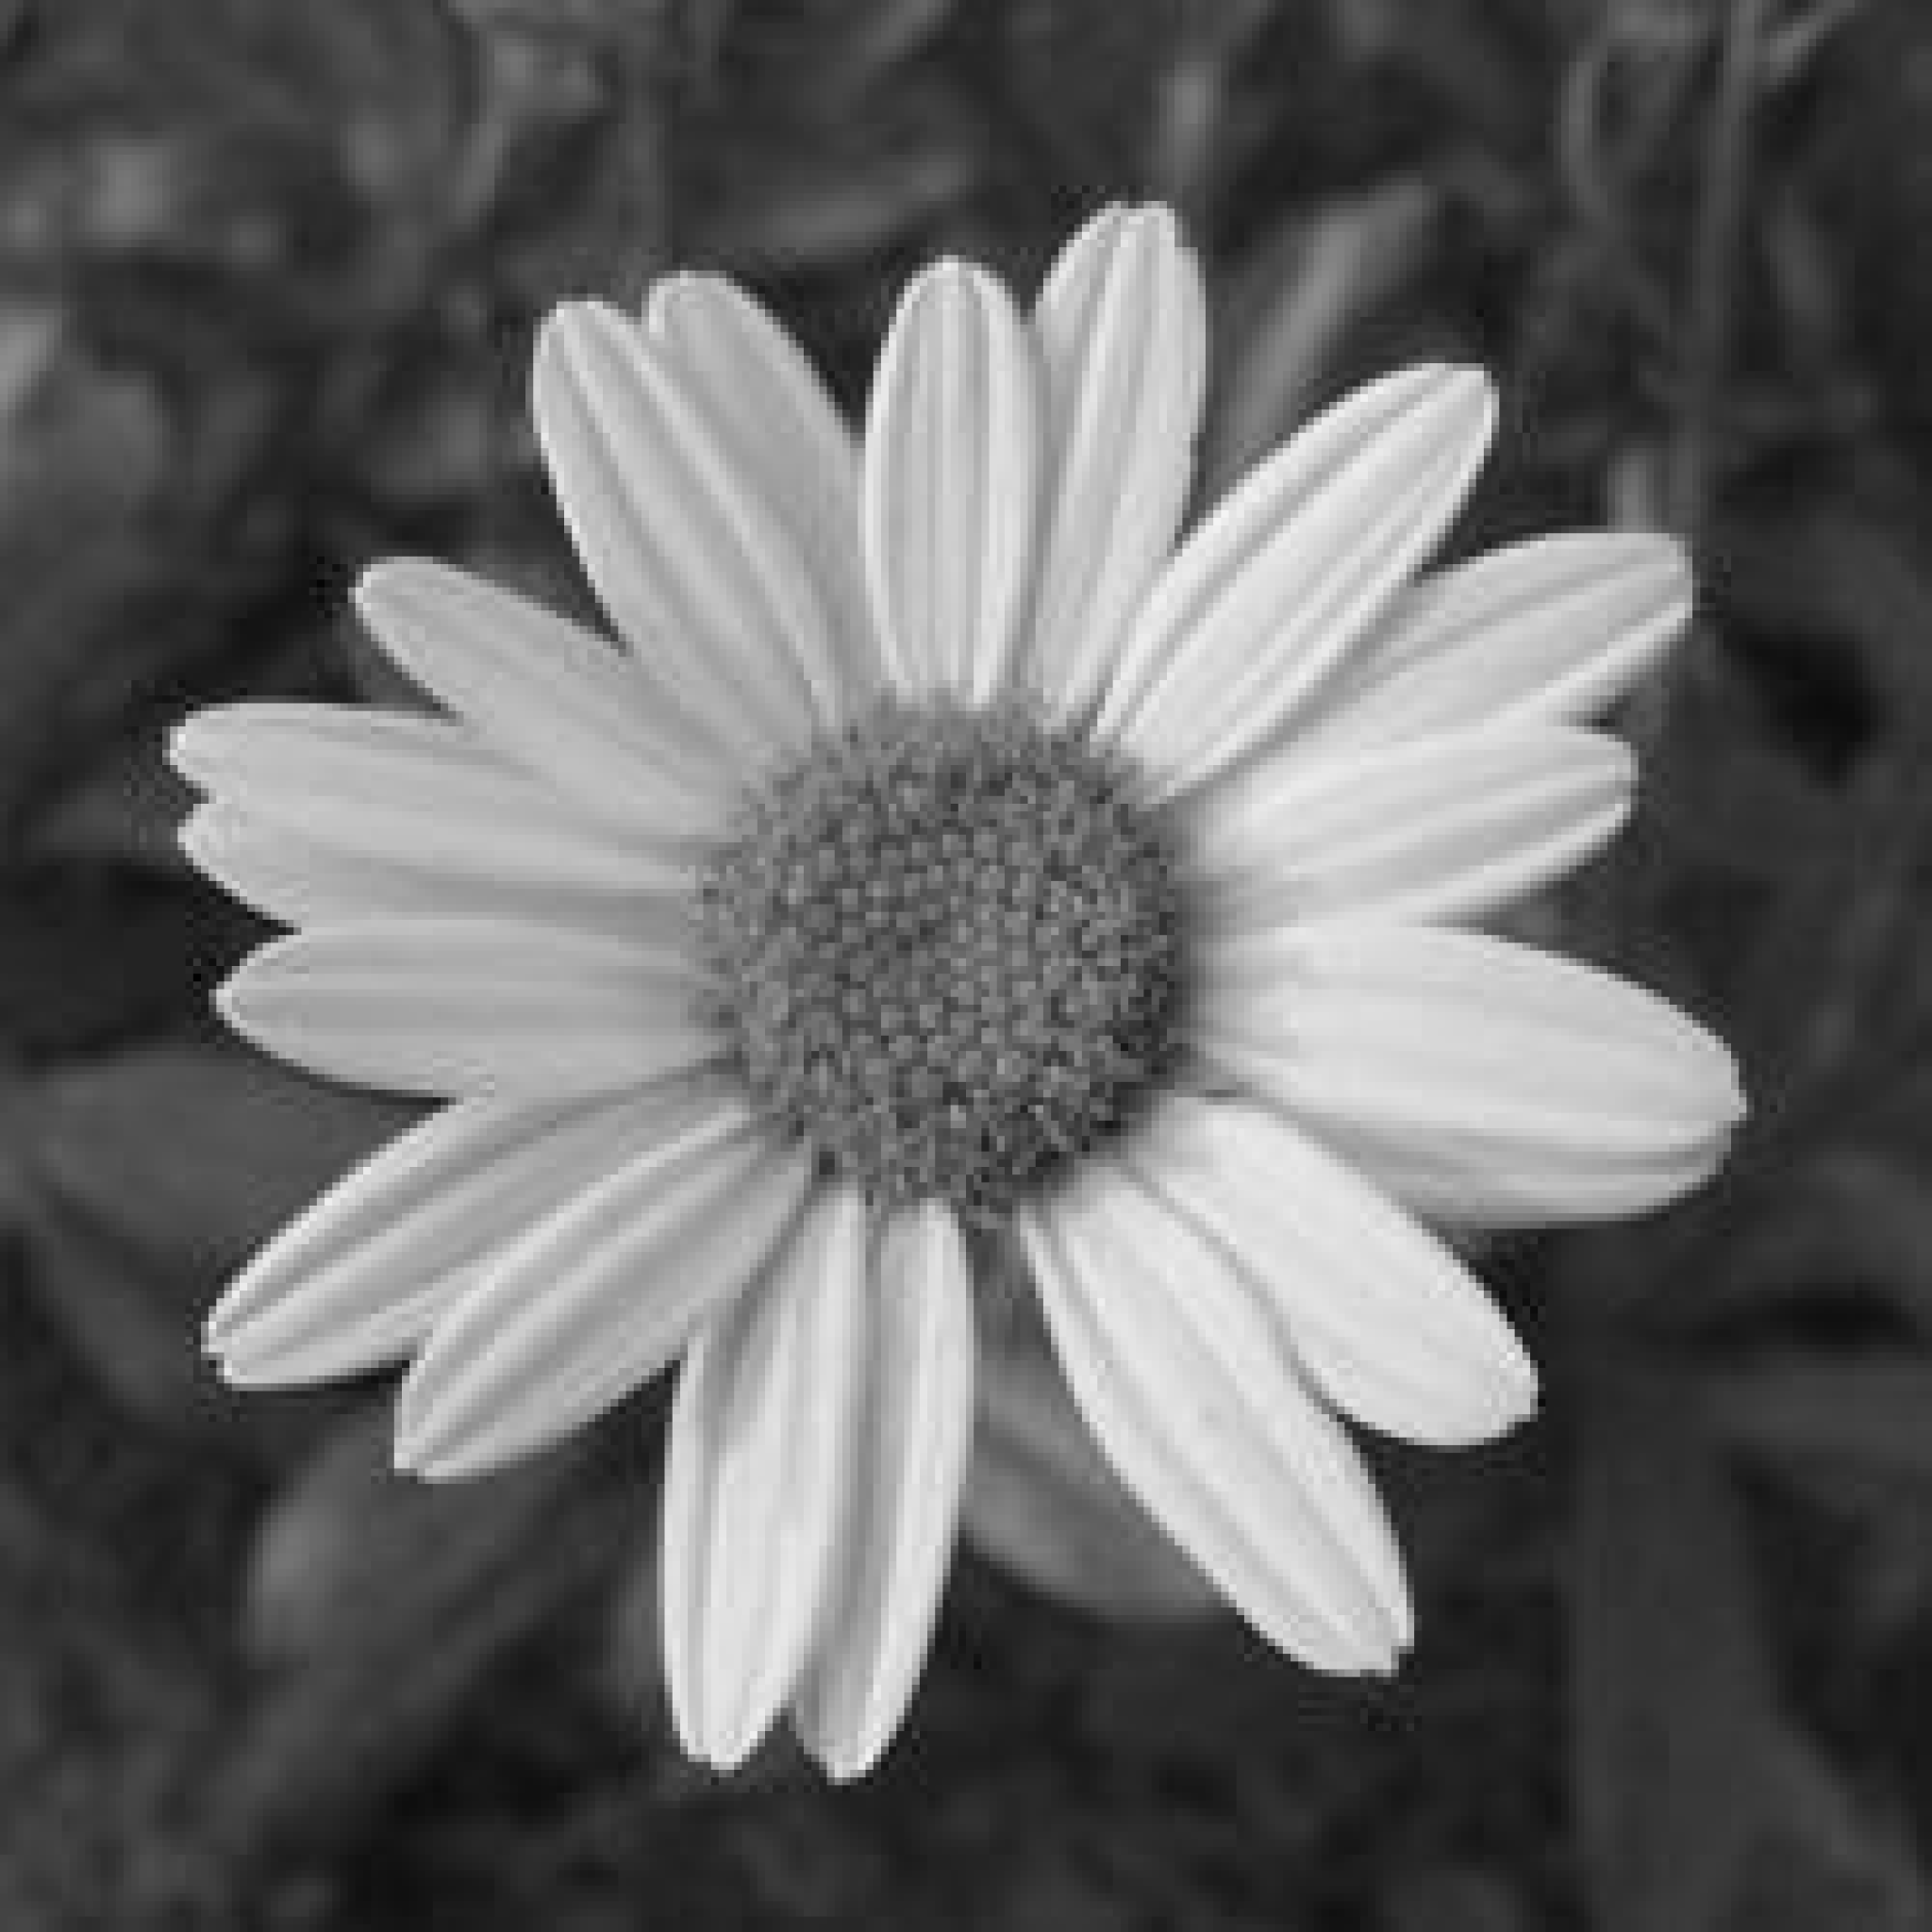
\includegraphics[interpolate=false, scale=0.08]{img/big_orig} }} \\
    \subfloat[frecuencias]{{ 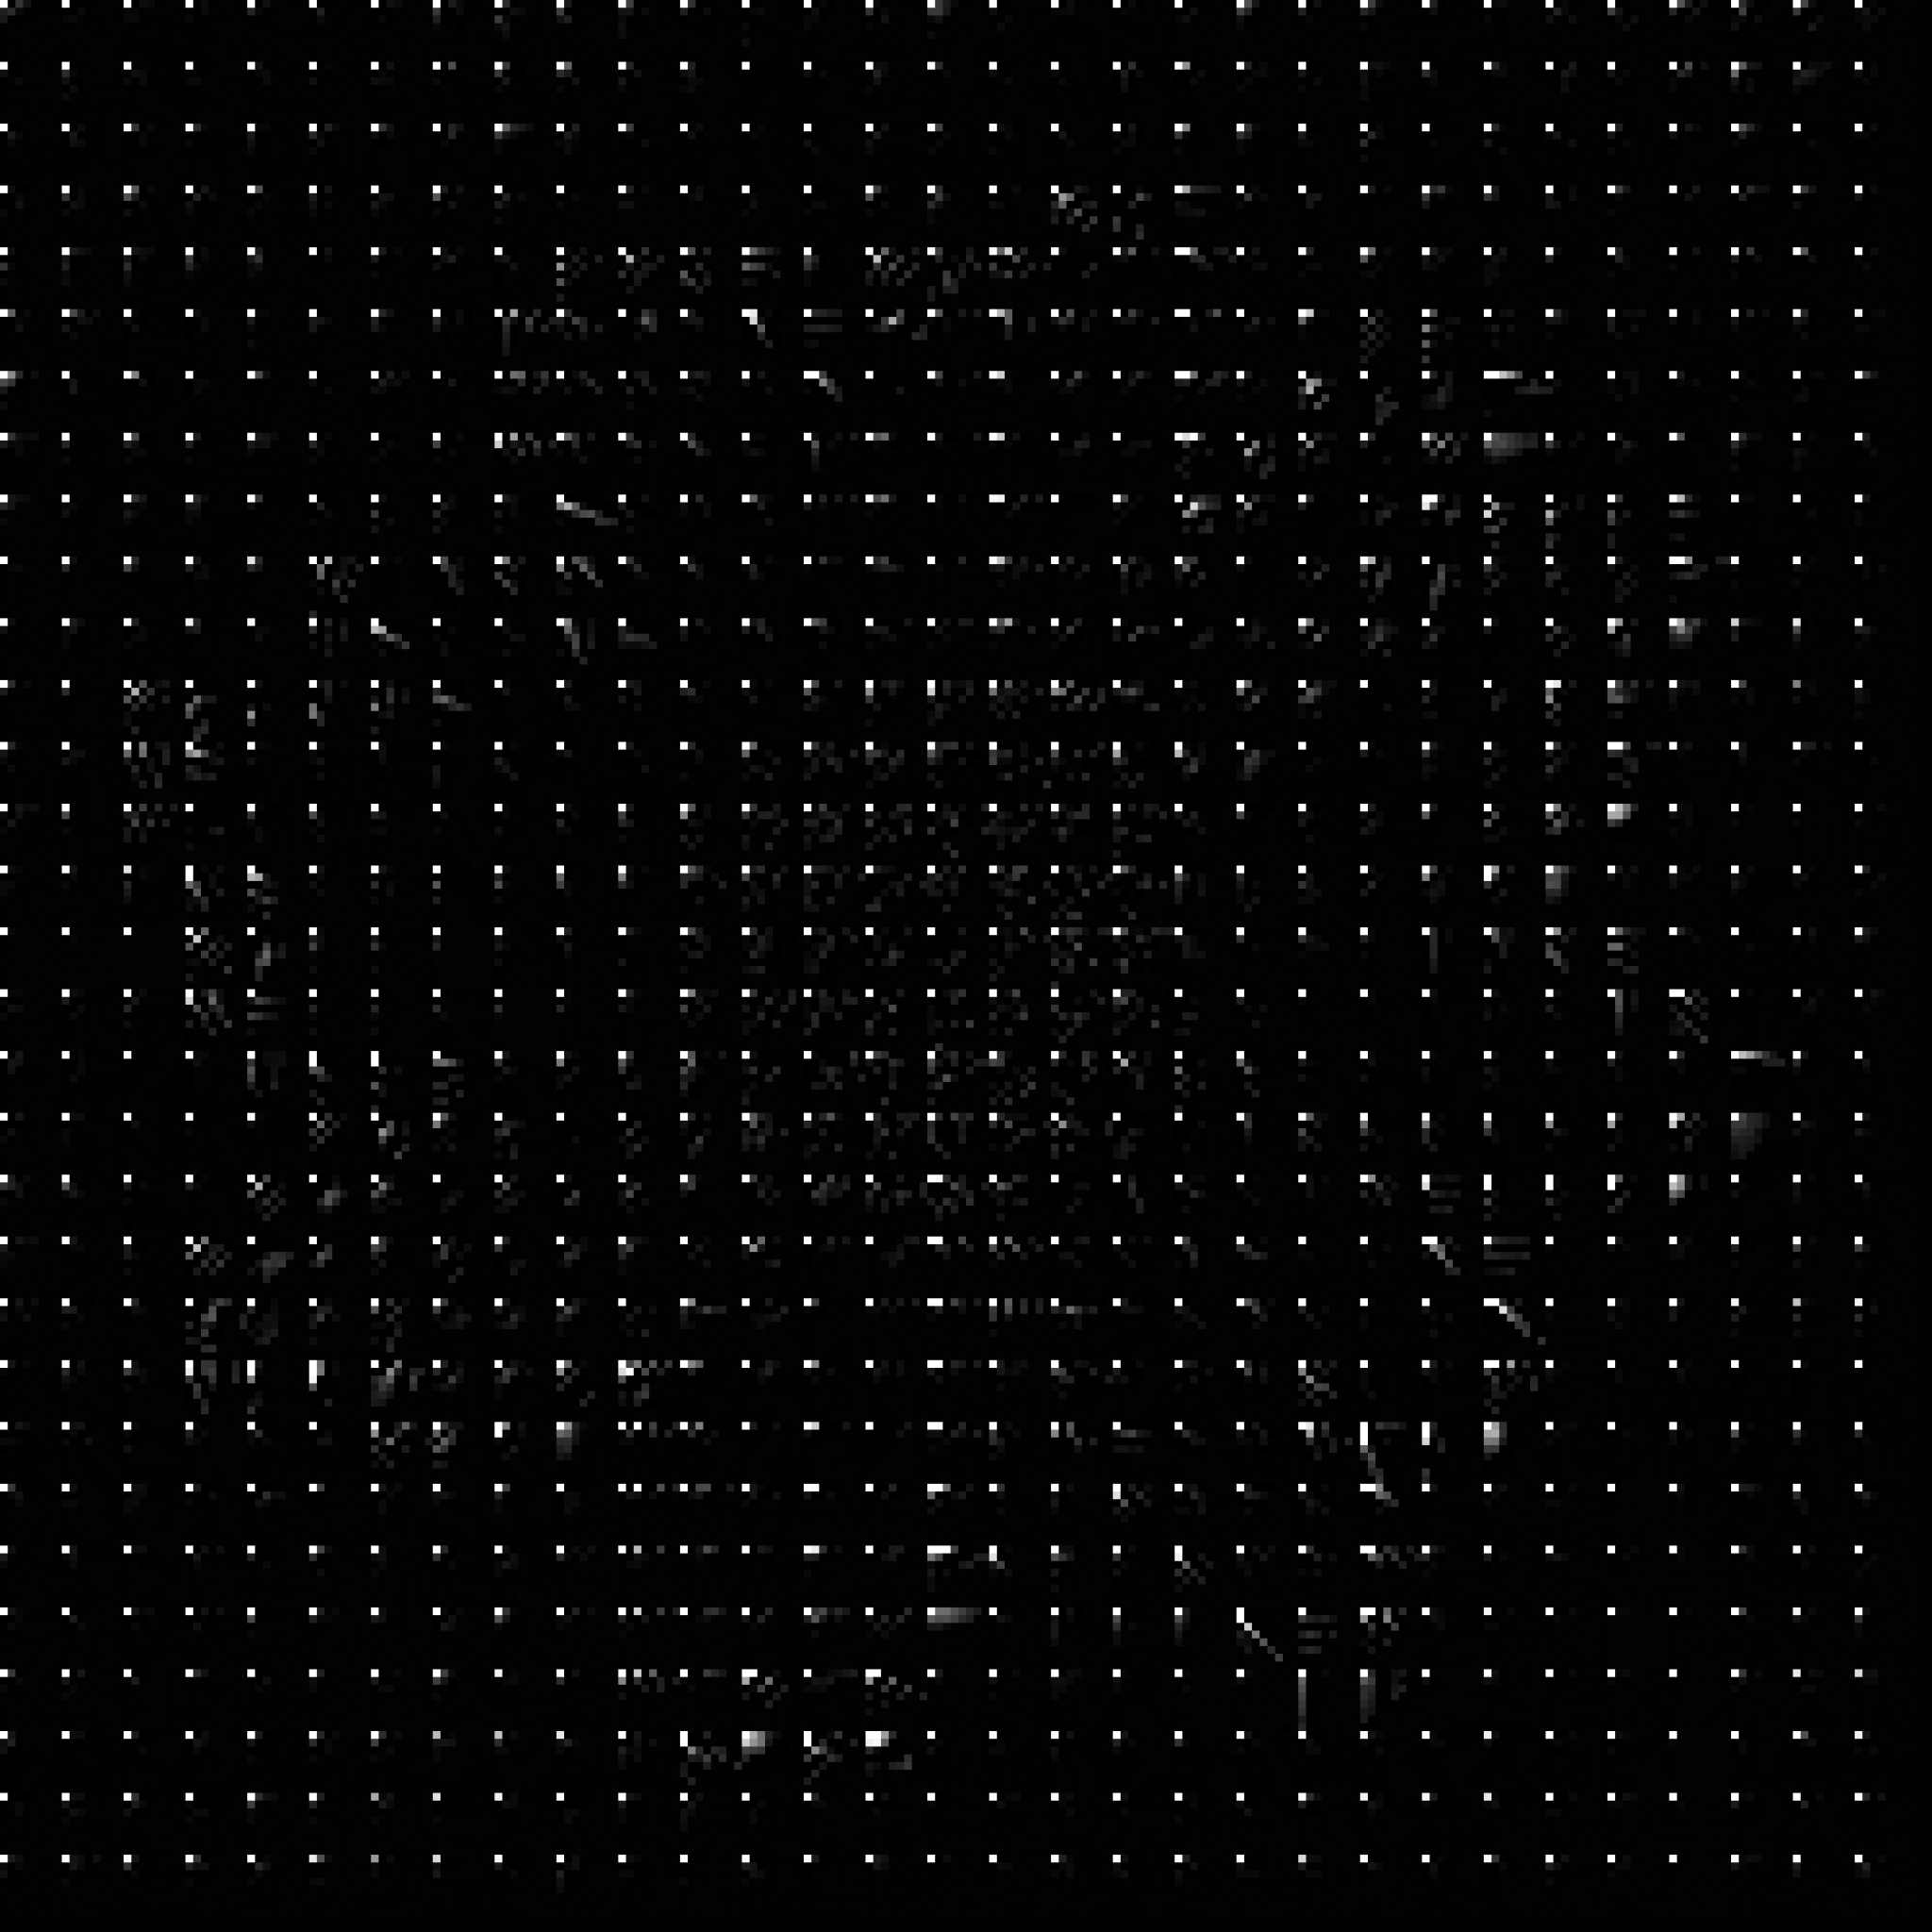
\includegraphics[interpolate=false, scale=0.08]{img/big_freq} }} \\
    \subfloat[recuperada]{{ 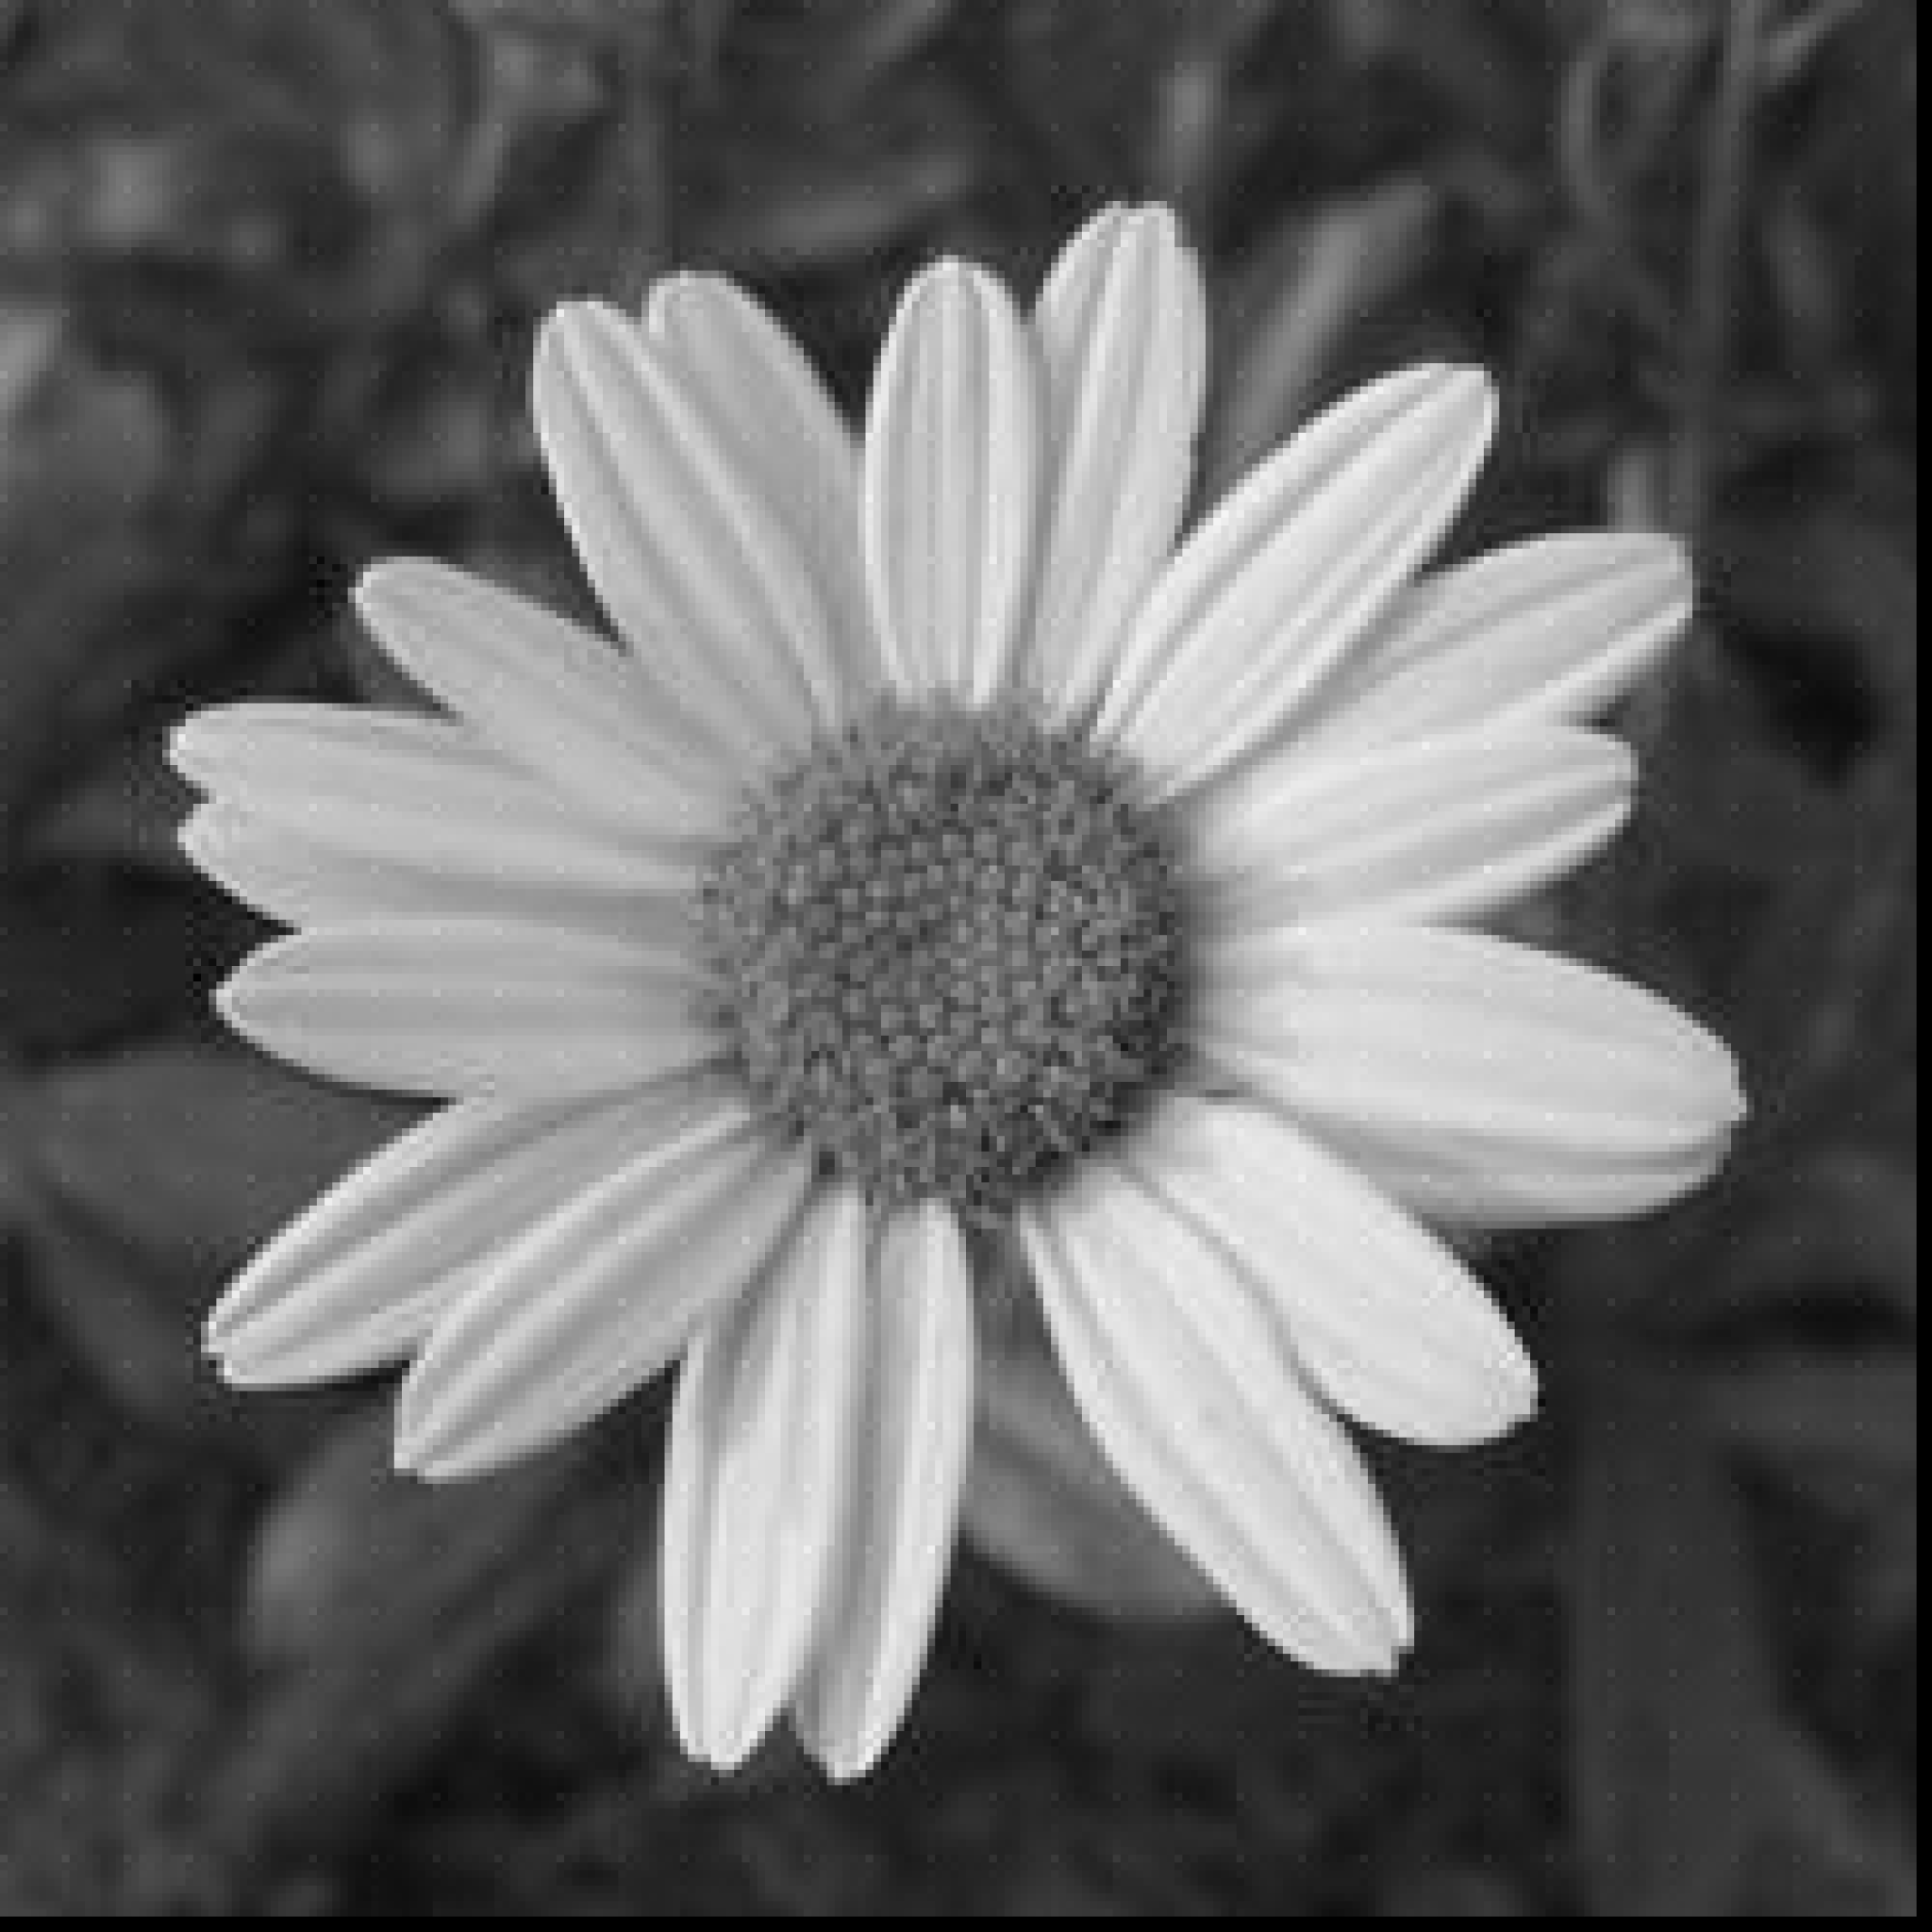
\includegraphics[interpolate=false, scale=0.08]{img/big_comp} }}
    \caption{Imágenes en el transcurso del algoritmo}
    \label{fig:original}
\end{figure}

%-- FILTERED MODERATE

\subsection{Filtro moderado}

Usando un filtro que retiene únicamente un sector de las frecuencias logramos una mejora en la compresión, pero al reconstruir la imagen utilizando la transformada inversa del coseno podemos notar un deterioro grande de la imagen.

\lstinputlisting[style=Style1, firstline=11, lastline=25, caption=Matriz de filtro moderado, label=code:filter_m]{src/runner.py}

\begin{lstlisting}[language=bash]
make flower
env/bin/python src/runner.py source_images/04_flower.png
Running image:  source_images/04_flower.png
Compression gain: 27.49 %
\end{lstlisting}

\begin{figure}[!htbp]
    \centering
    \subfloat[no filtrada]{{ 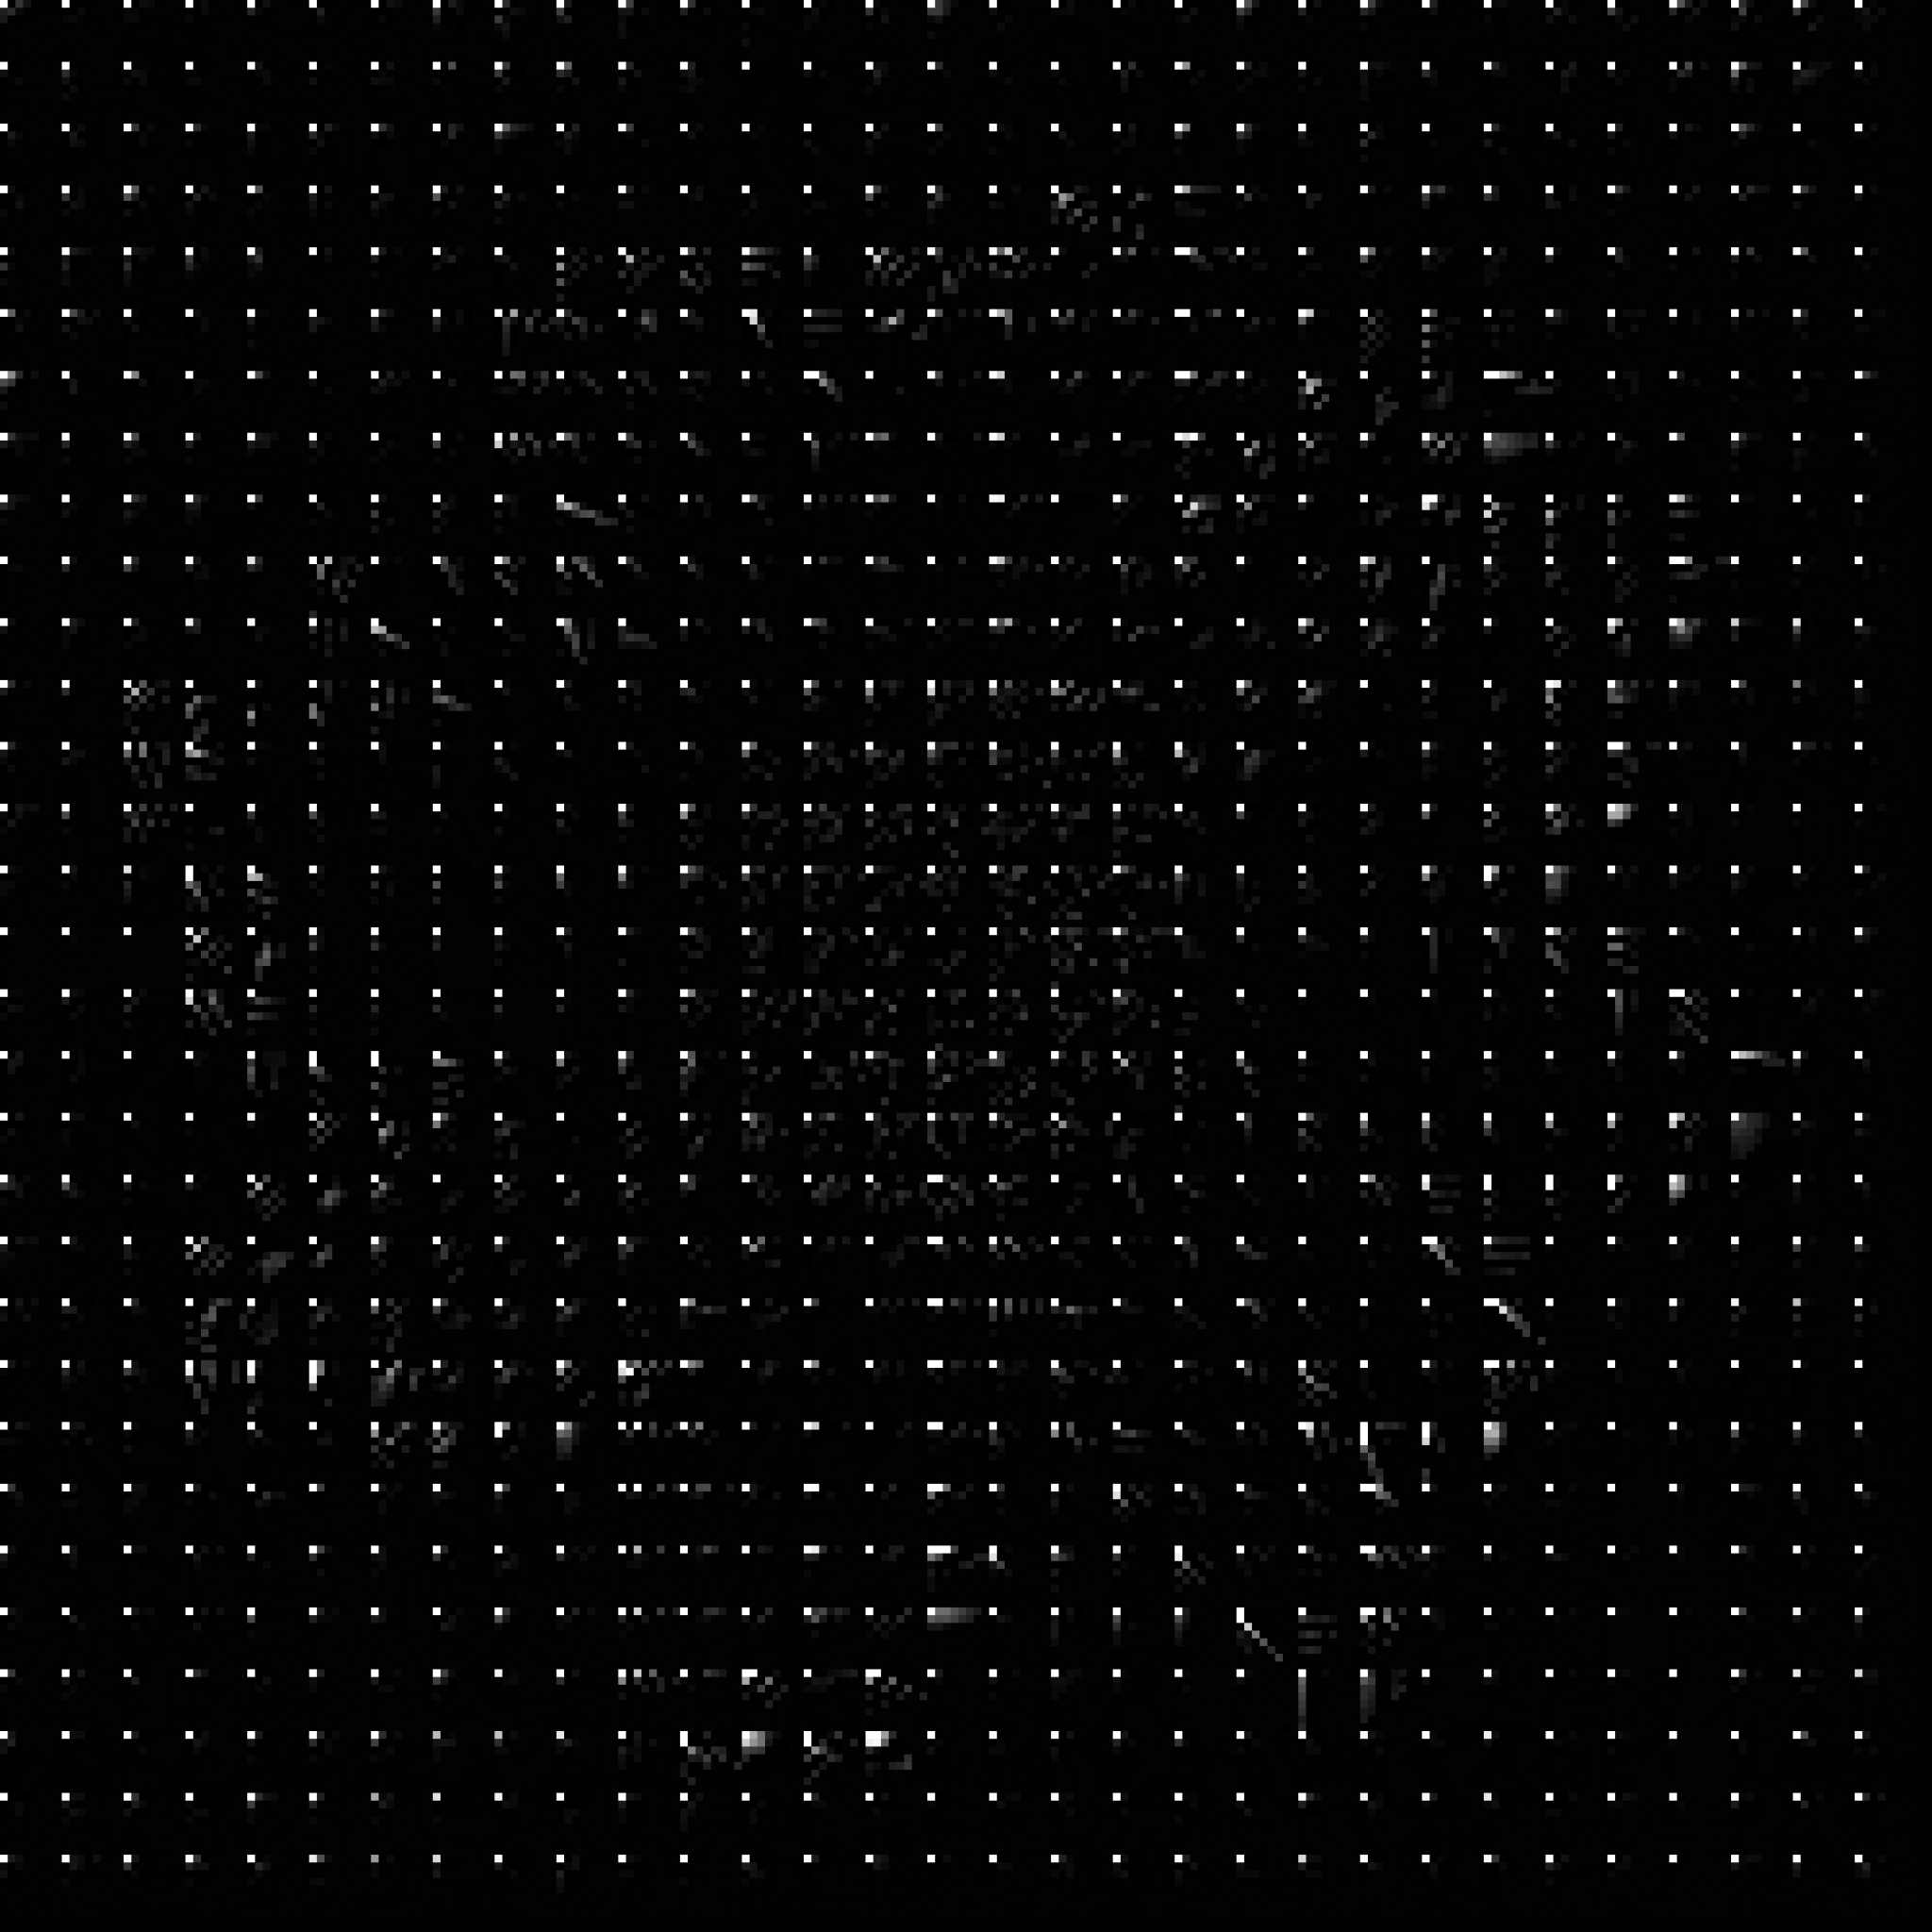
\includegraphics[interpolate=false, scale=0.09]{img/big_freq} }}
    \qquad
    \subfloat[moderadamente filtrada]{{ 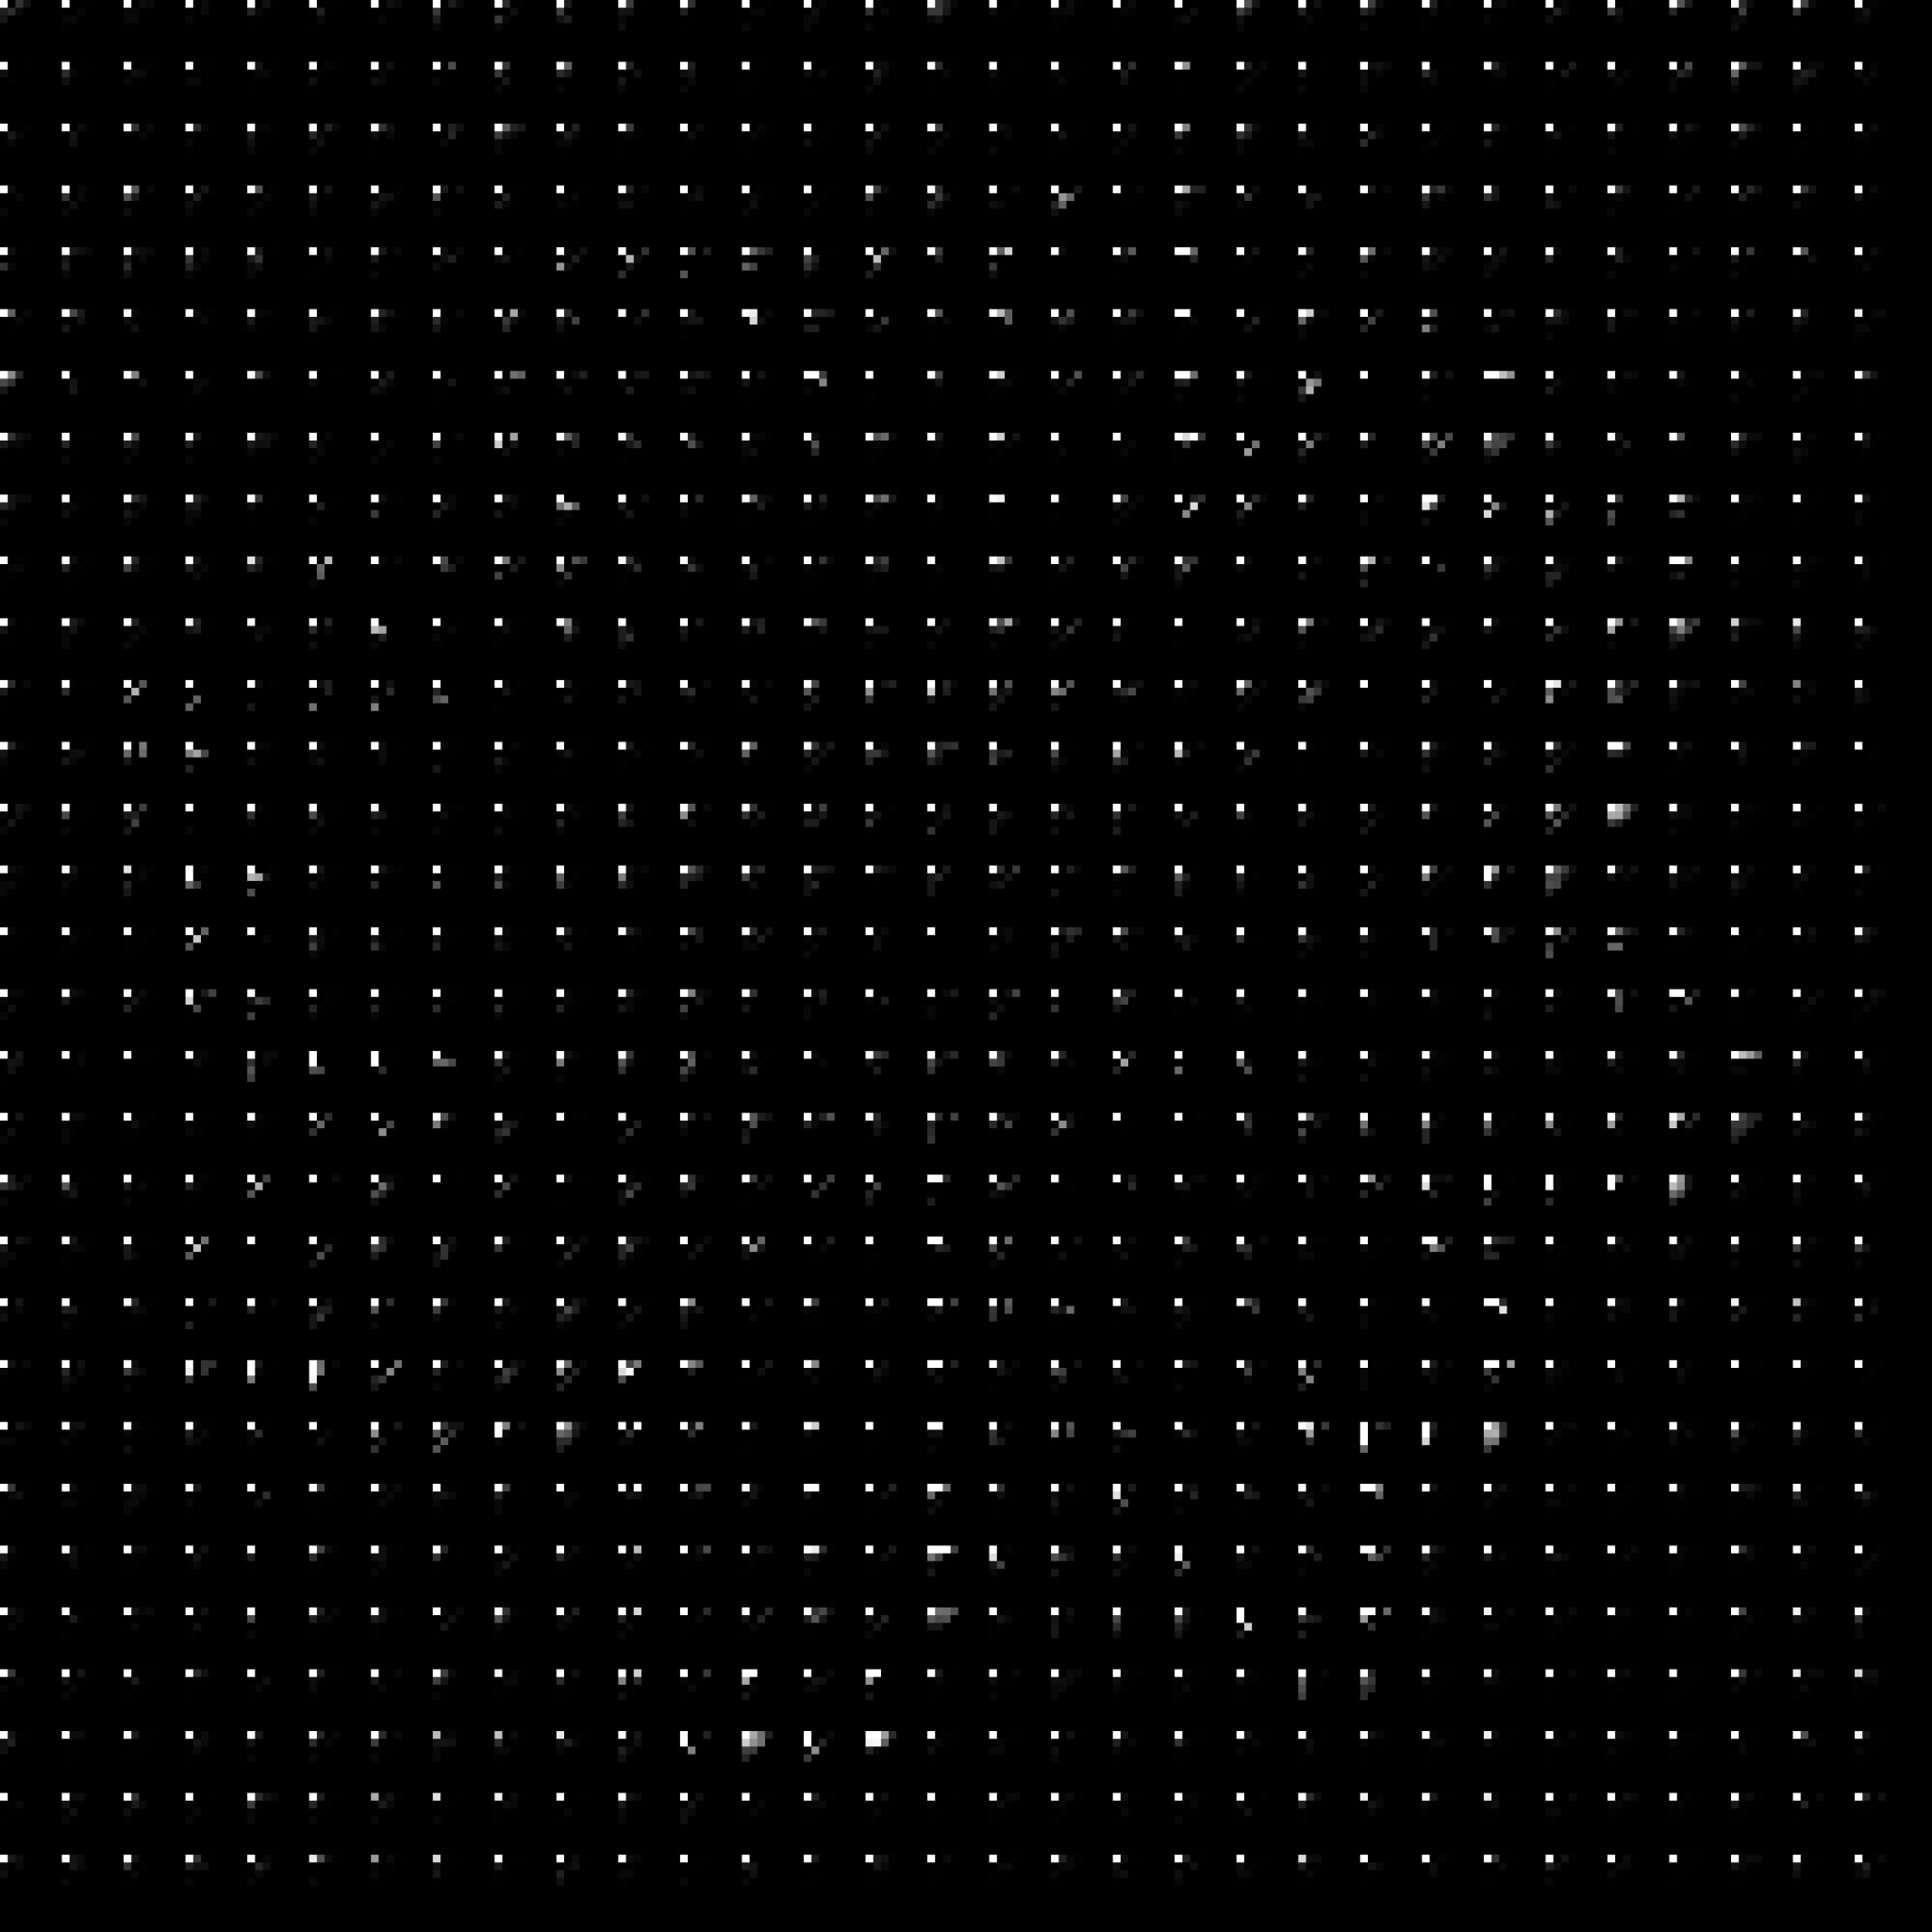
\includegraphics[interpolate=false, scale=0.09]{img/big_freq_fm} }}
    \caption{Comparación de imágenes de frecuencias}
    \label{fig:freq_fm}
\end{figure}

\begin{figure}[!htbp]
    \centering
    \subfloat[no filtrada]{{ 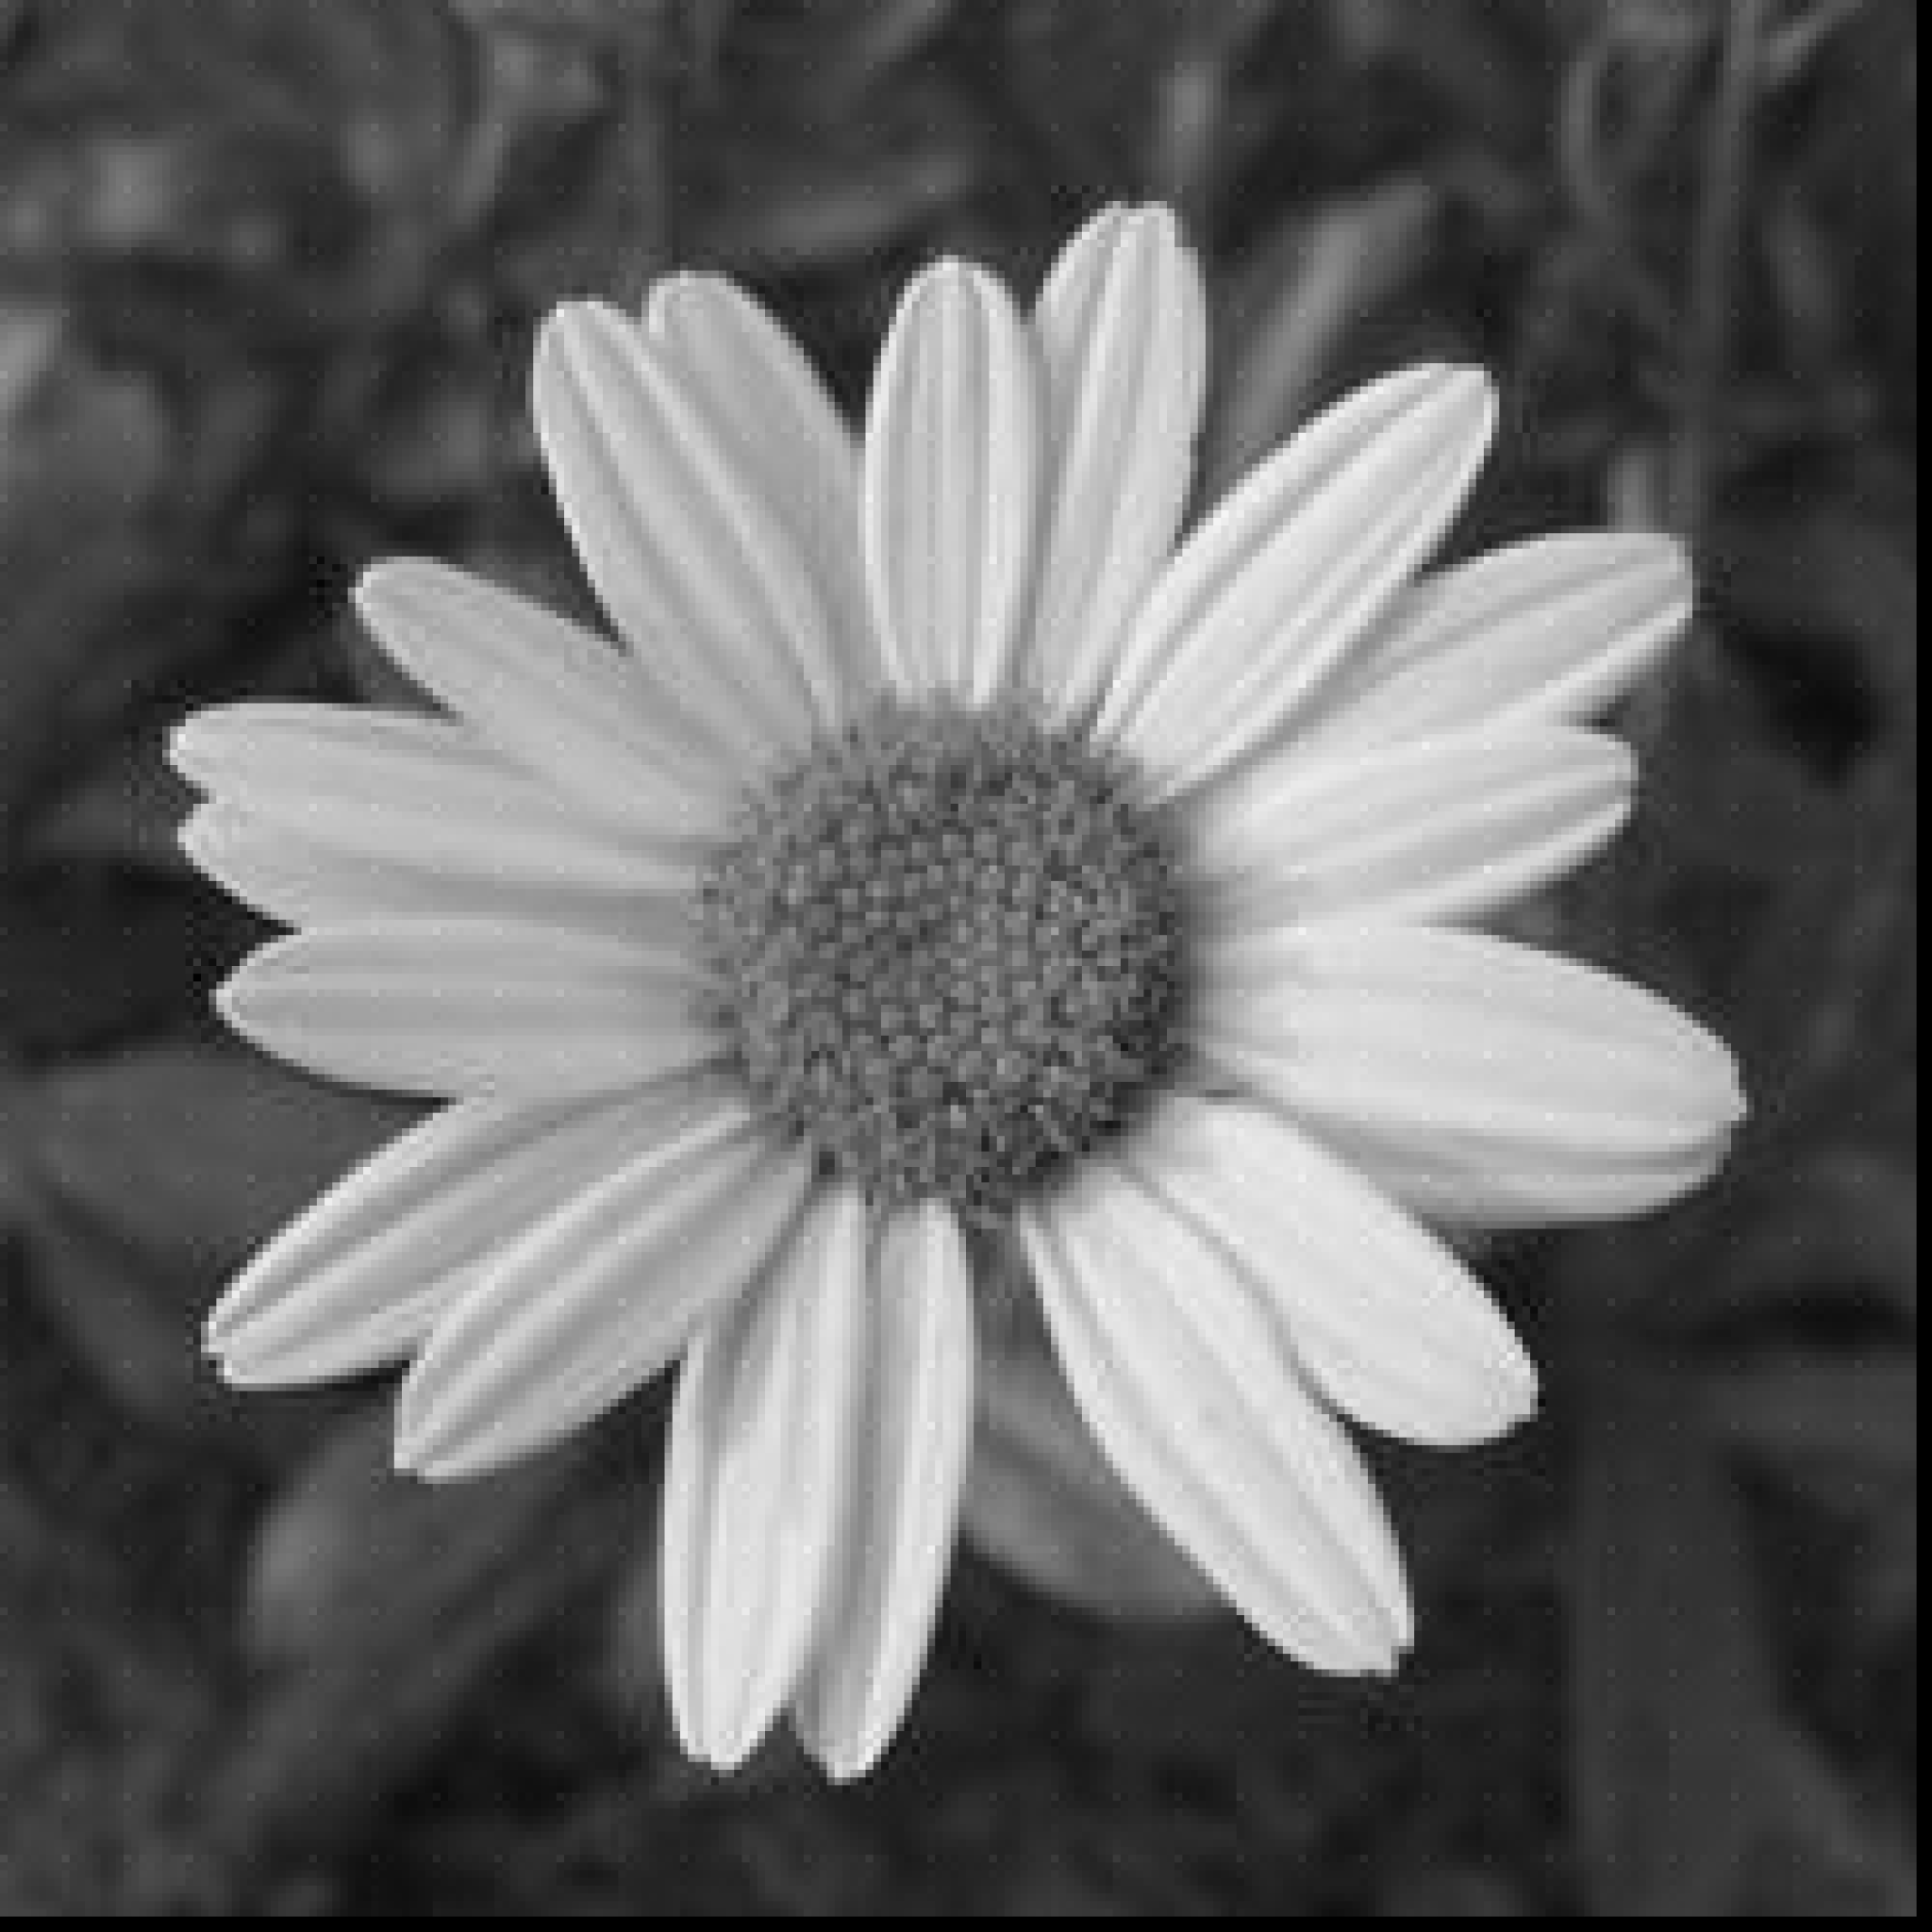
\includegraphics[interpolate=false, scale=0.09]{img/big_comp} }}
    \qquad
    \subfloat[moderadamente filtrada]{{ 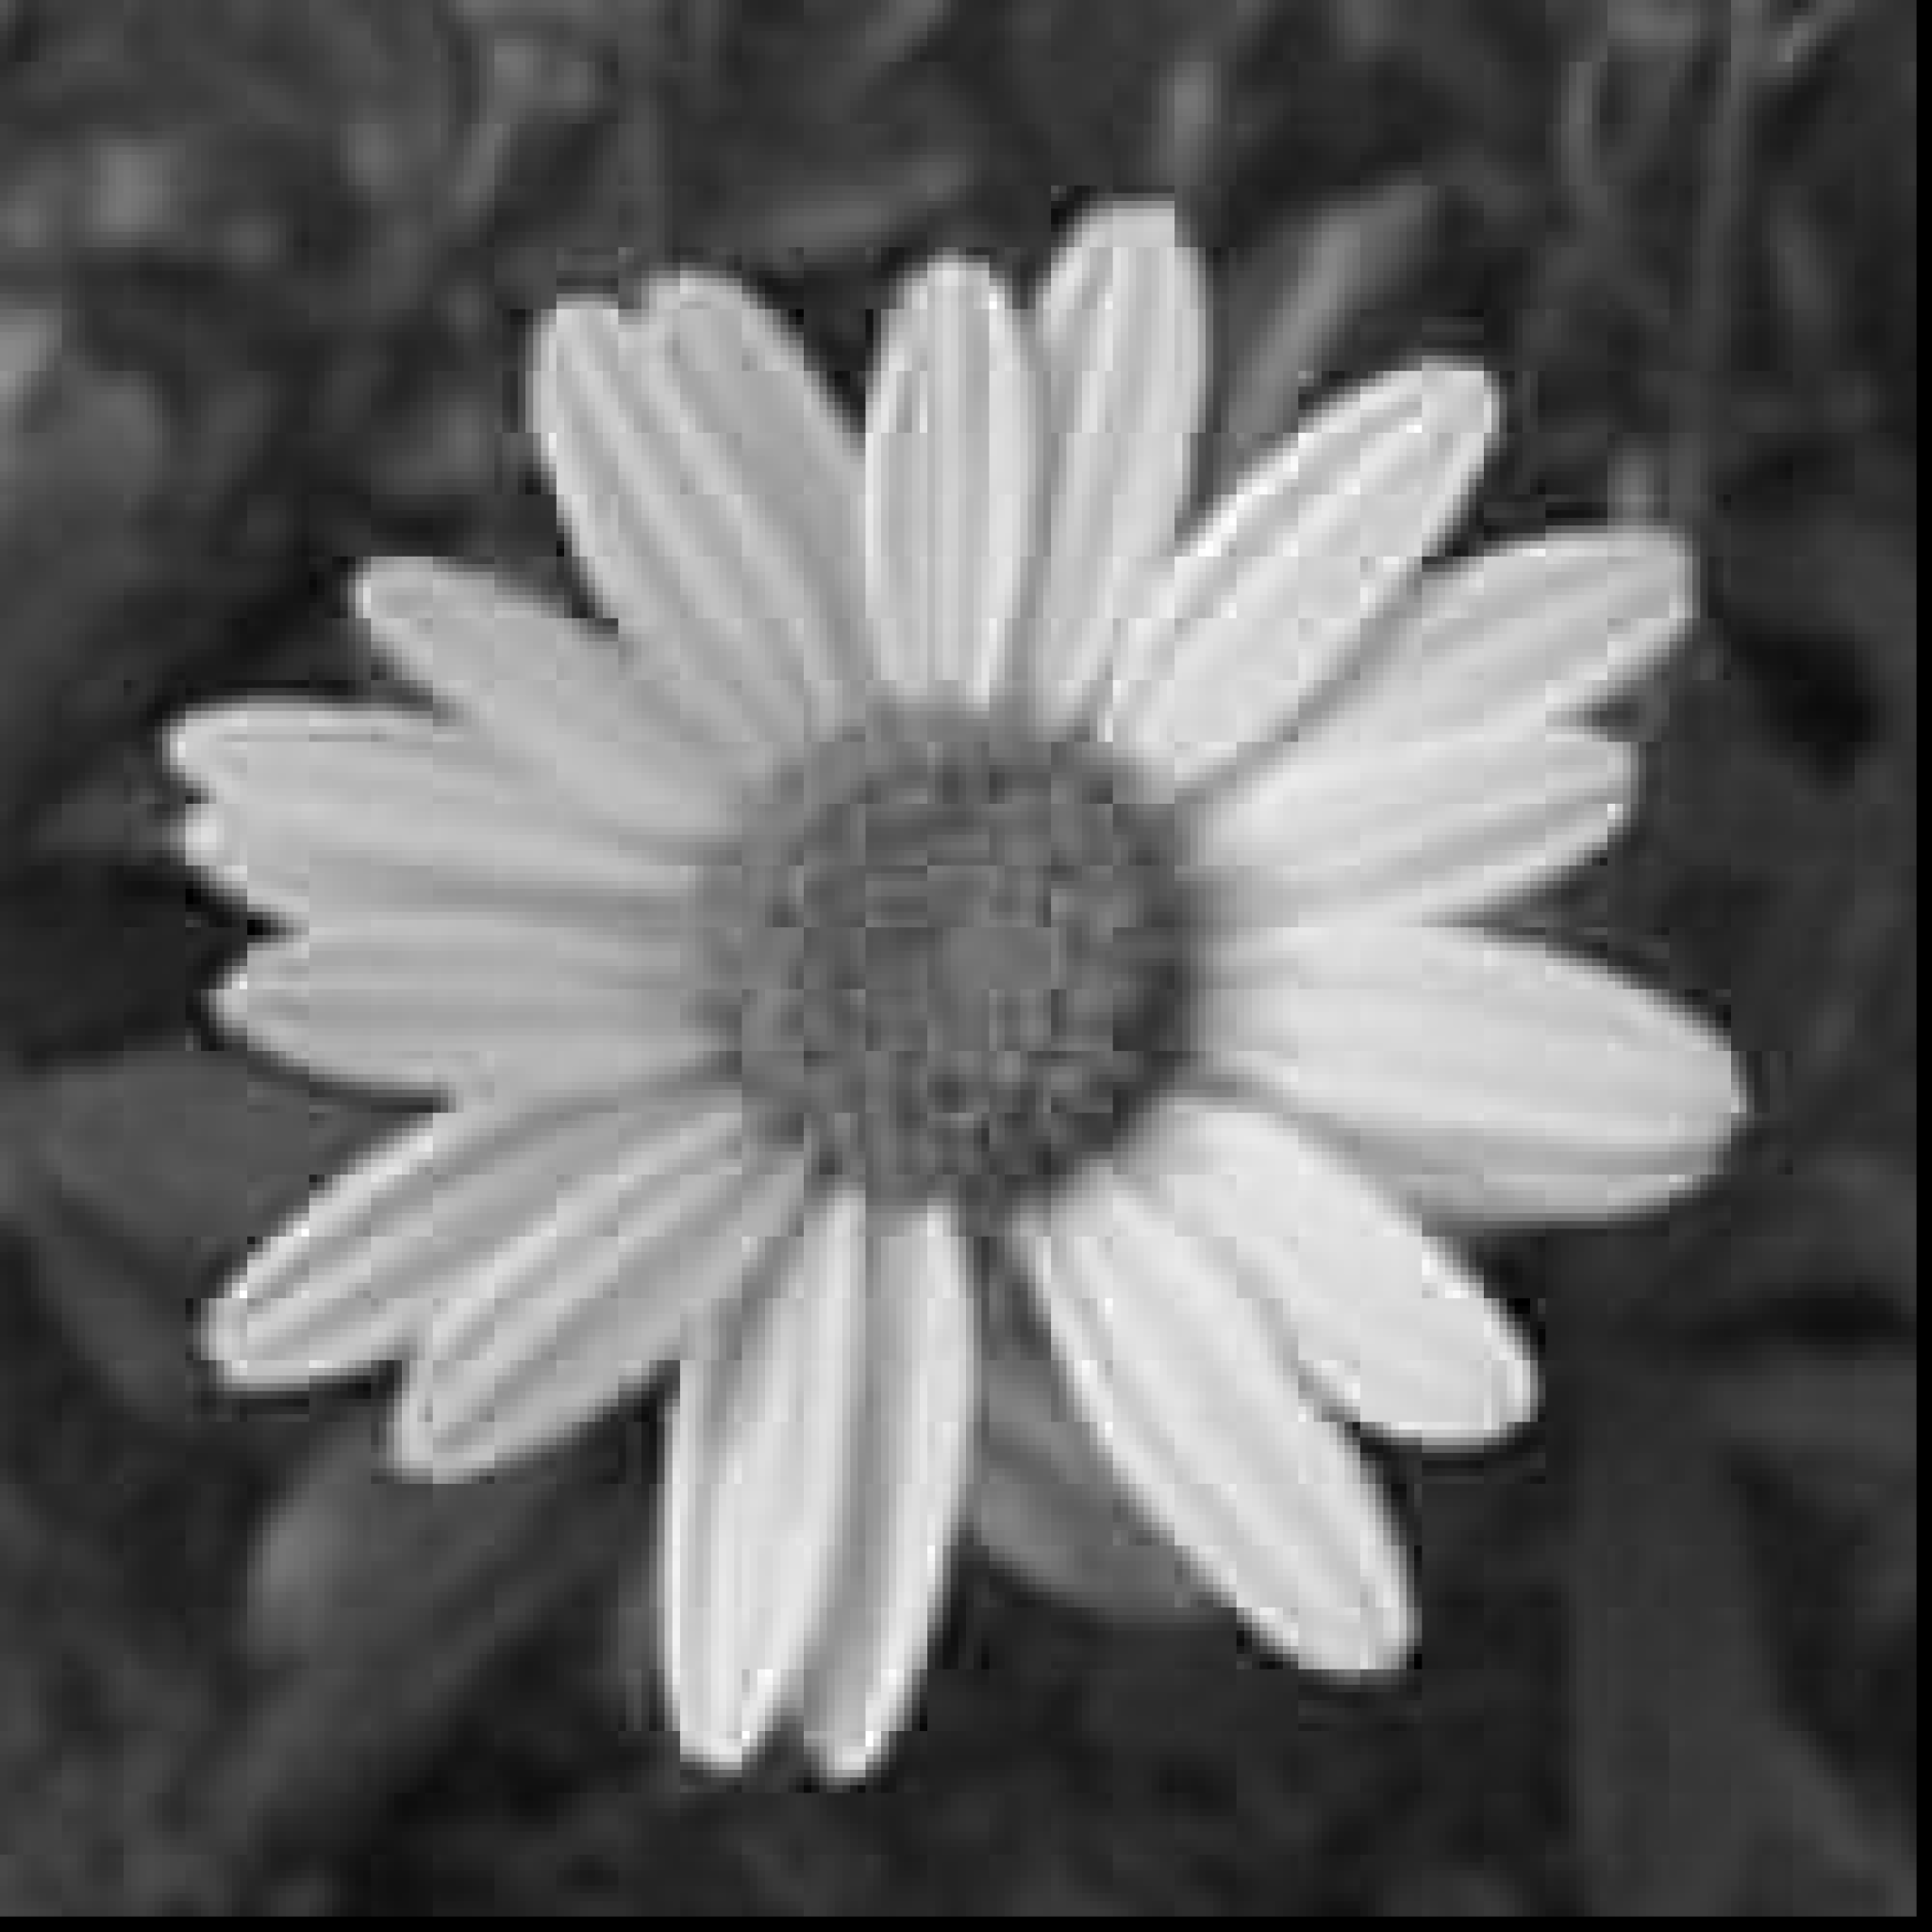
\includegraphics[interpolate=false, scale=0.09]{img/big_comp_fm} }}
    \caption{Comparación de imágenes}
    \label{fig:comp_fm}
\end{figure}

%-- FILTERED HEAVY

\subsection{Filtro pesado}

Al aplicar un filtro más agresivo (descartar todos salvo un elemento de las frecuencias generadas en cada bloque por el algoritmo de la transformada discreta del coseno) notamos una compresión enorme (92.29\%). Sin embargo, la imagen se encuentra totalmente deteriorada dado que en cada sector de 8x8 hay un solo color.
\lstinputlisting[style=Style1, firstline=28, lastline=42, caption=Matriz de filtro pesado, label=code:filter_h]{src/runner.py}

\begin{lstlisting}[language=bash]
make flower
env/bin/python src/runner.py source_images/04_flower.png
Running image:  source_images/04_flower.png
Compression gain: 92.29 %
\end{lstlisting}

\begin{figure}[!htbp]
    \centering
    \subfloat[no filtrada]{{ 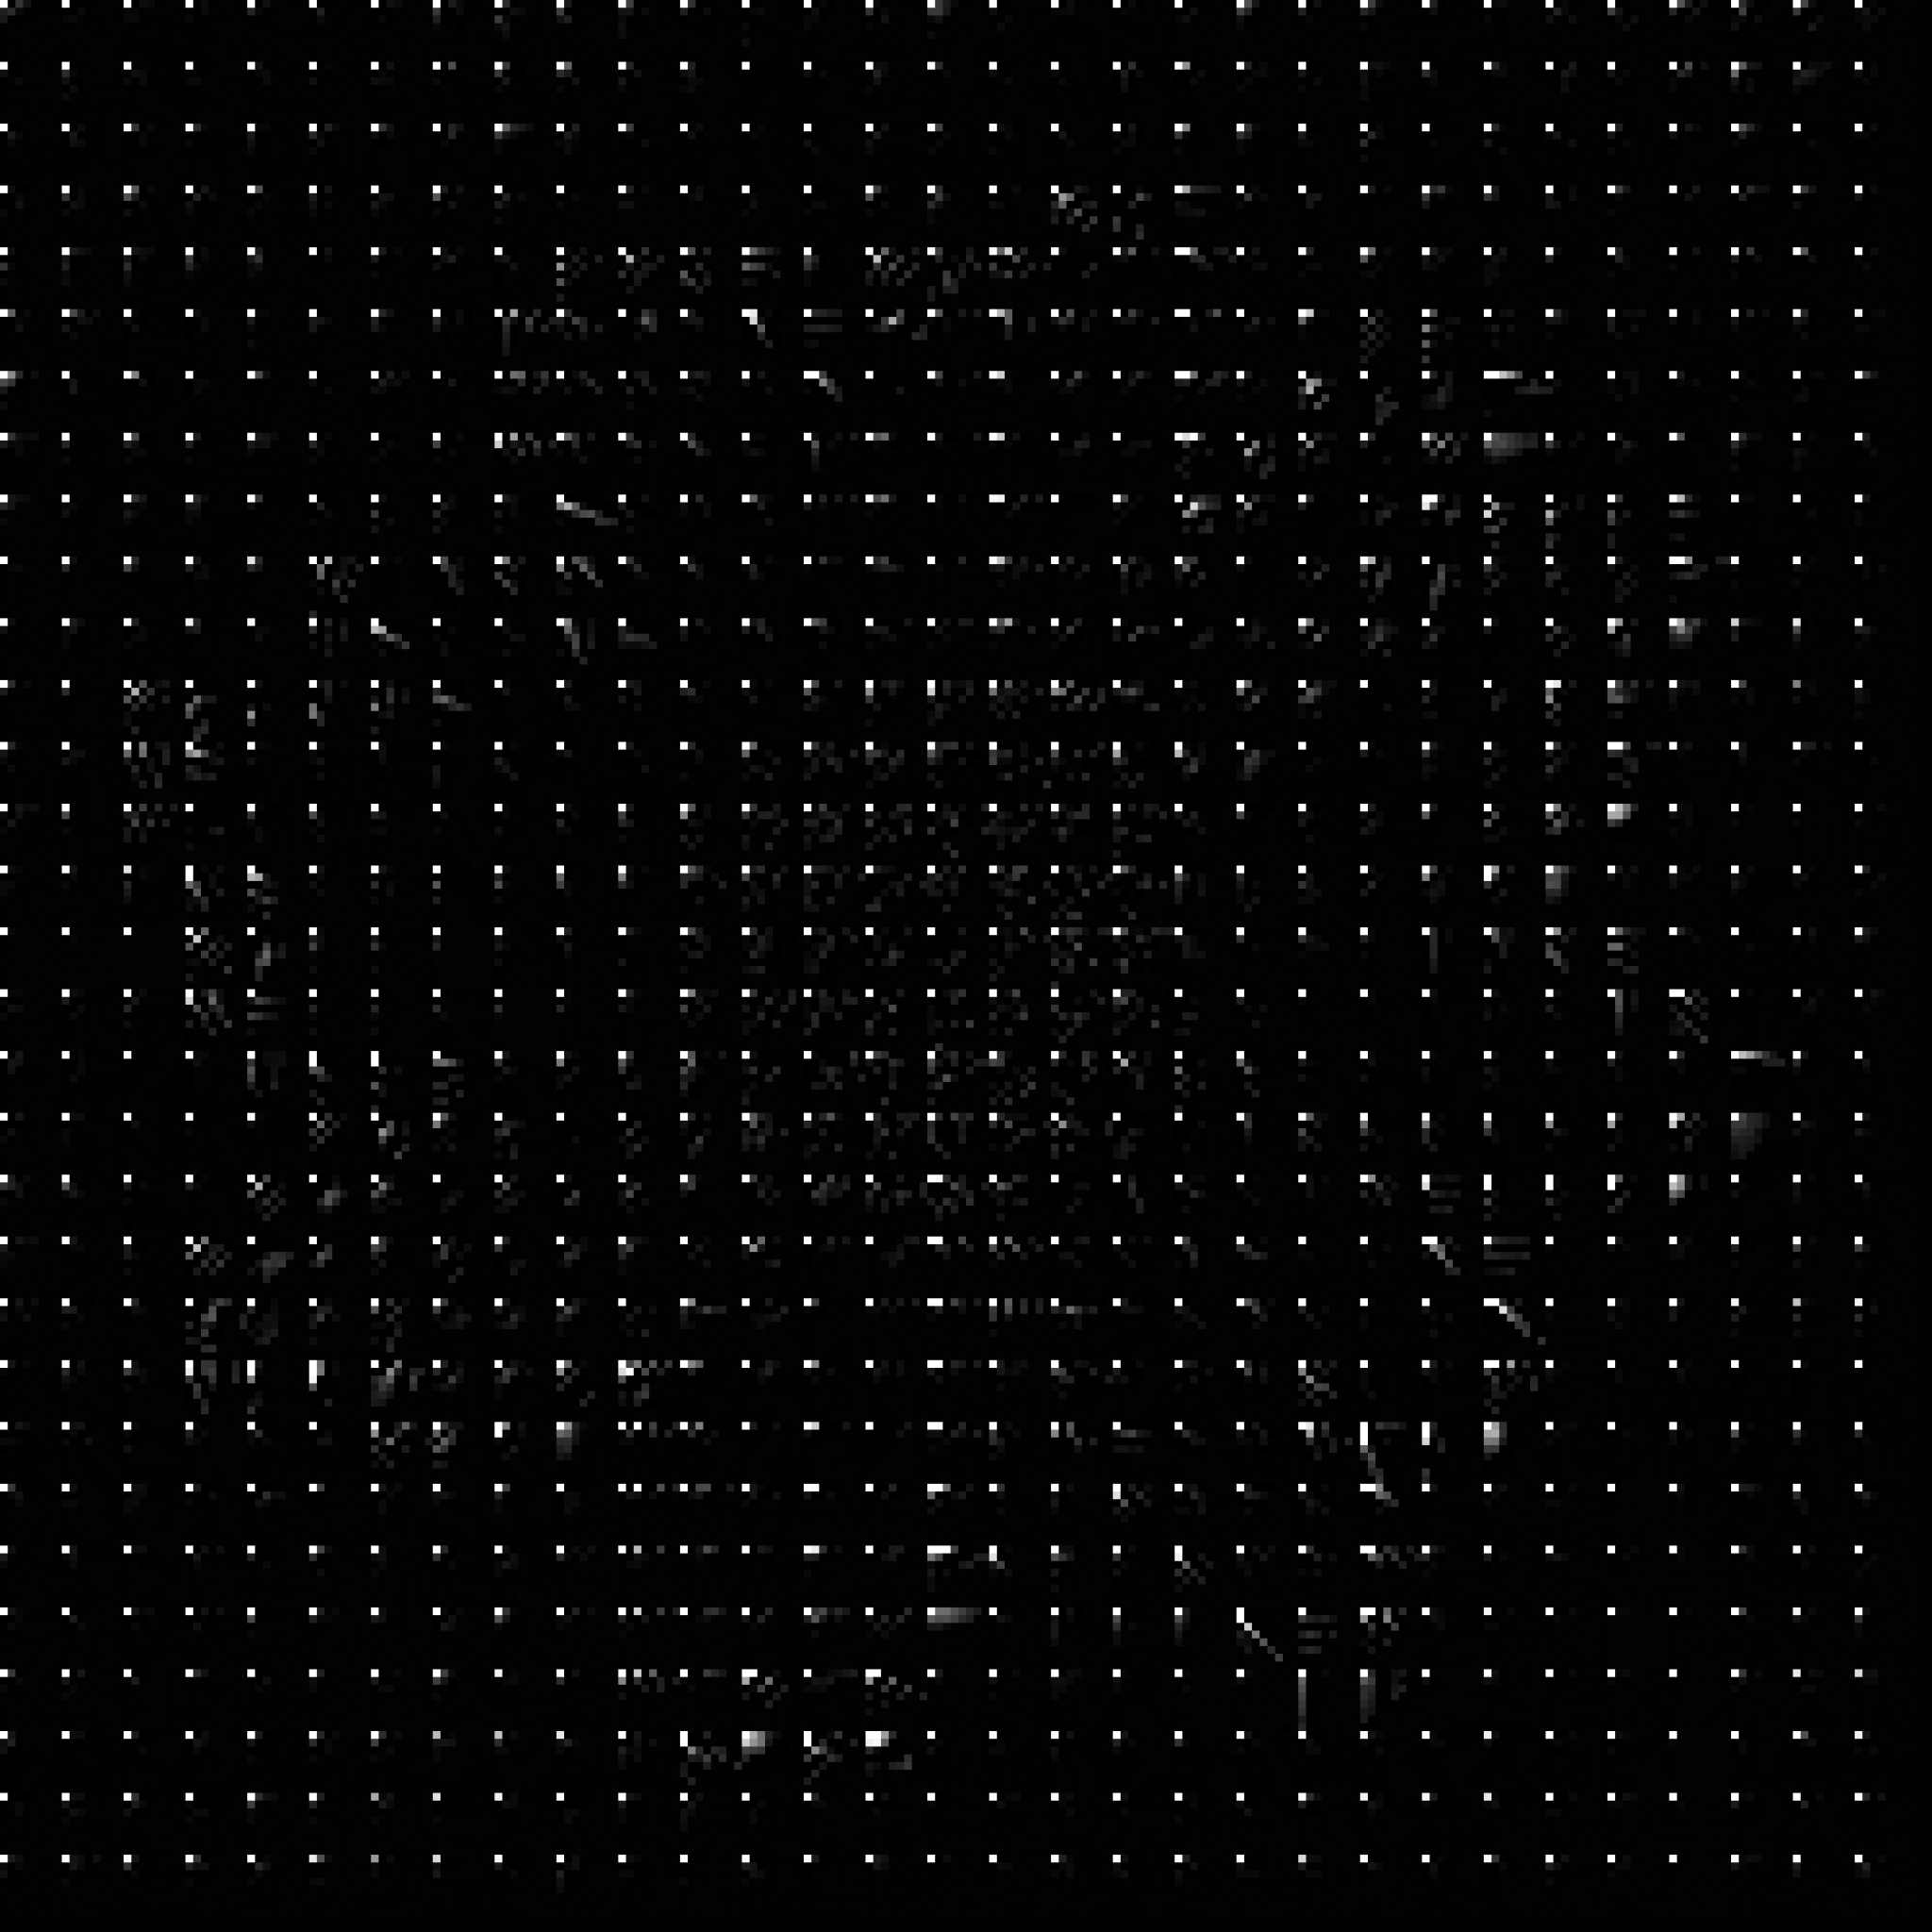
\includegraphics[interpolate=false, scale=0.09]{img/big_freq} }}
    \qquad
    \subfloat[muy filtrada]{{ 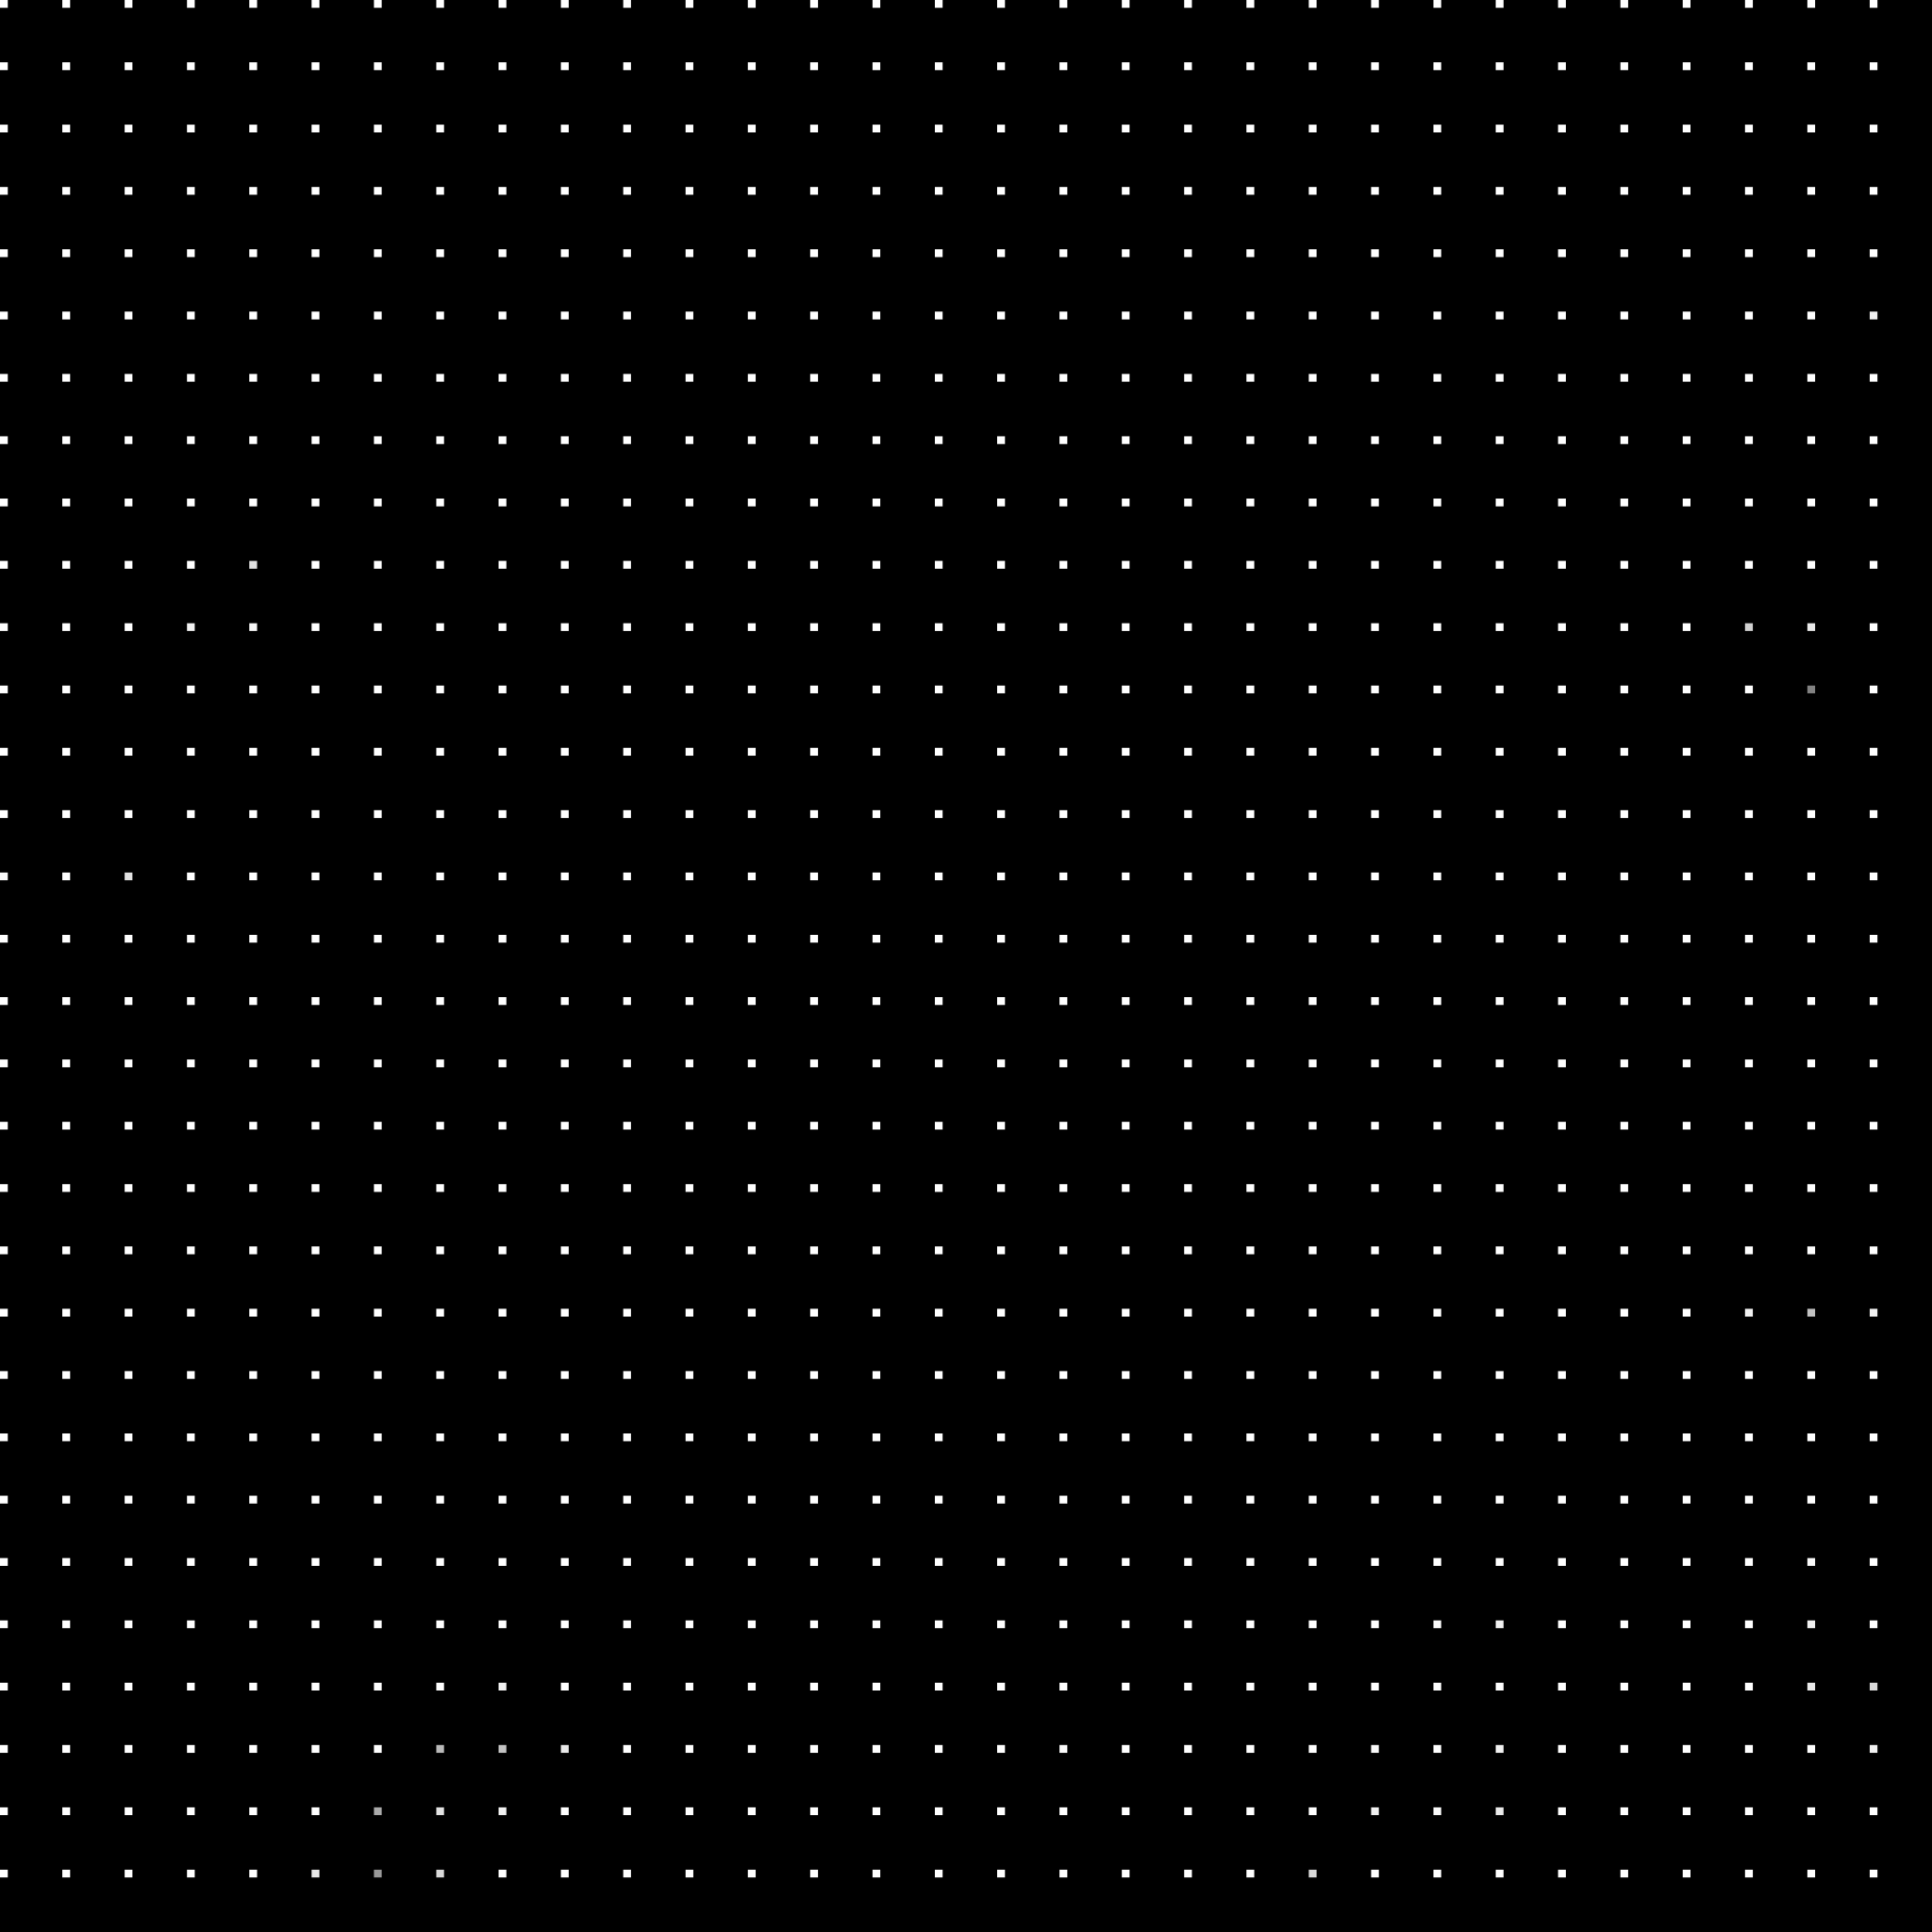
\includegraphics[interpolate=false, scale=0.09]{img/big_freq_fh} }}
    \caption{Comparacion de imagenes de frecuencias}
    \label{fig:freq_fh}
\end{figure}

\begin{figure}[!htbp]
    \centering
    \subfloat[no filtrada]{{ 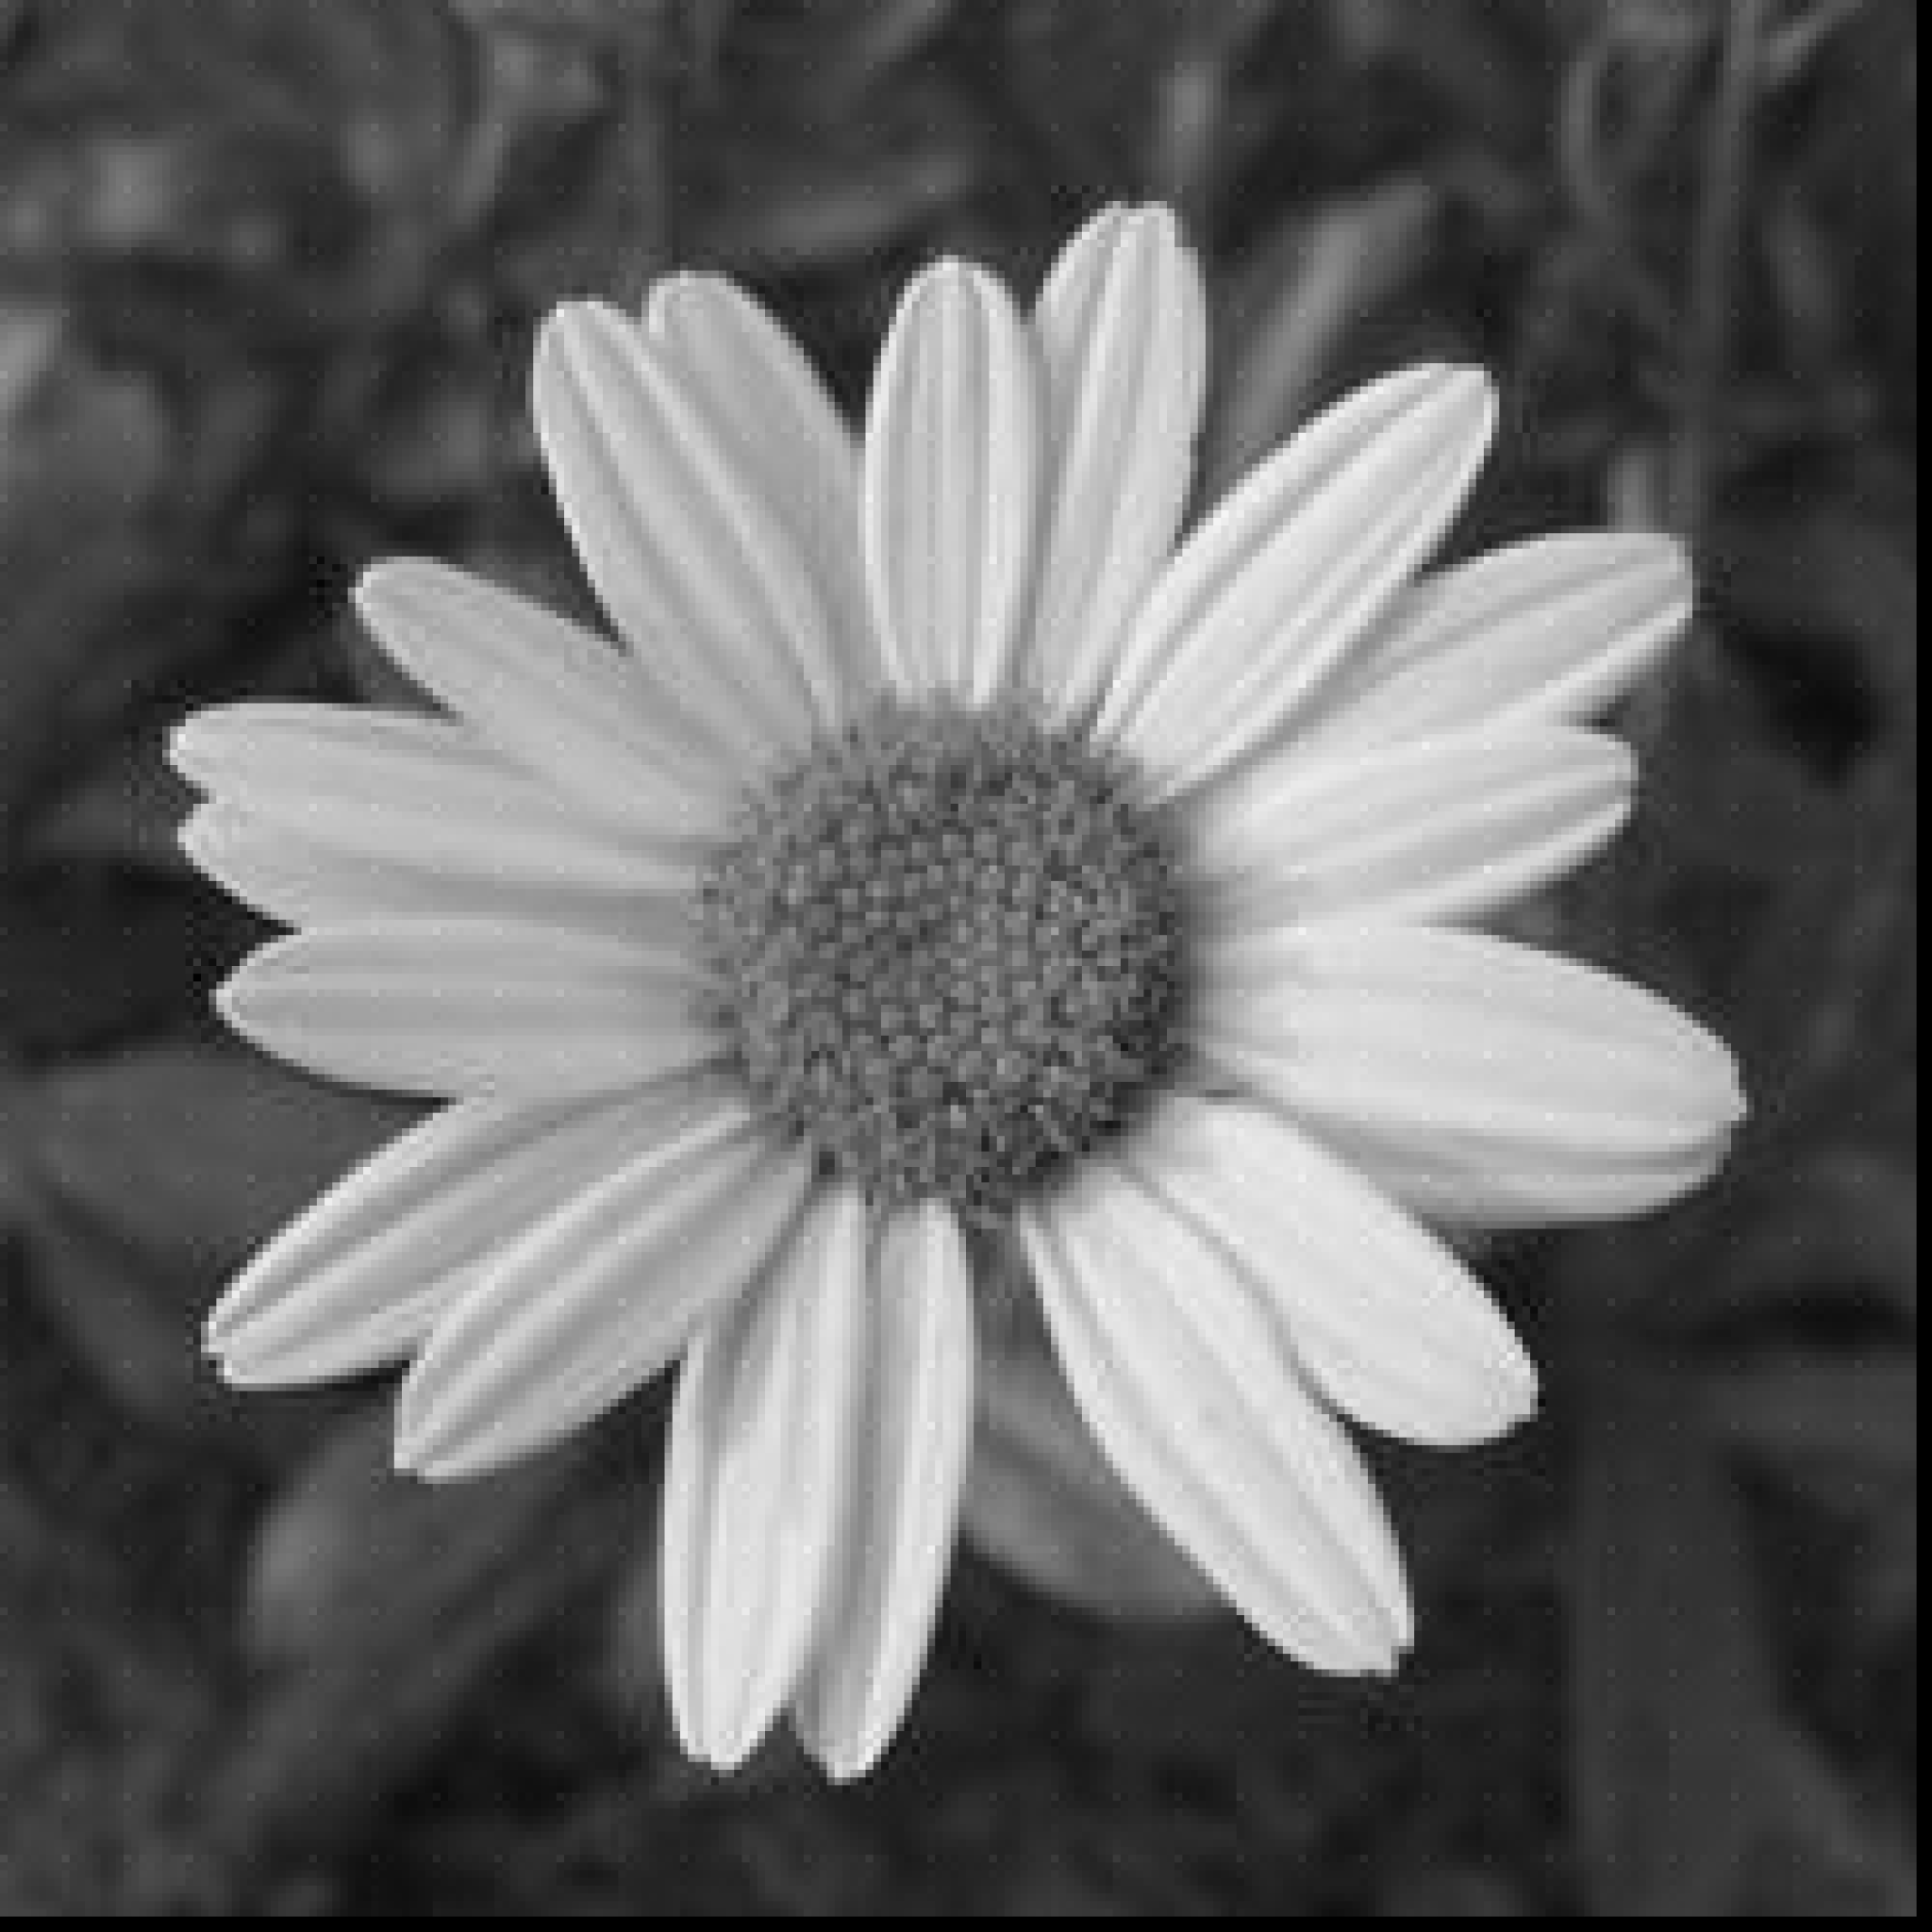
\includegraphics[interpolate=false, scale=0.09]{img/big_comp} }}
    \qquad
    \subfloat[muy filtrada]{{ 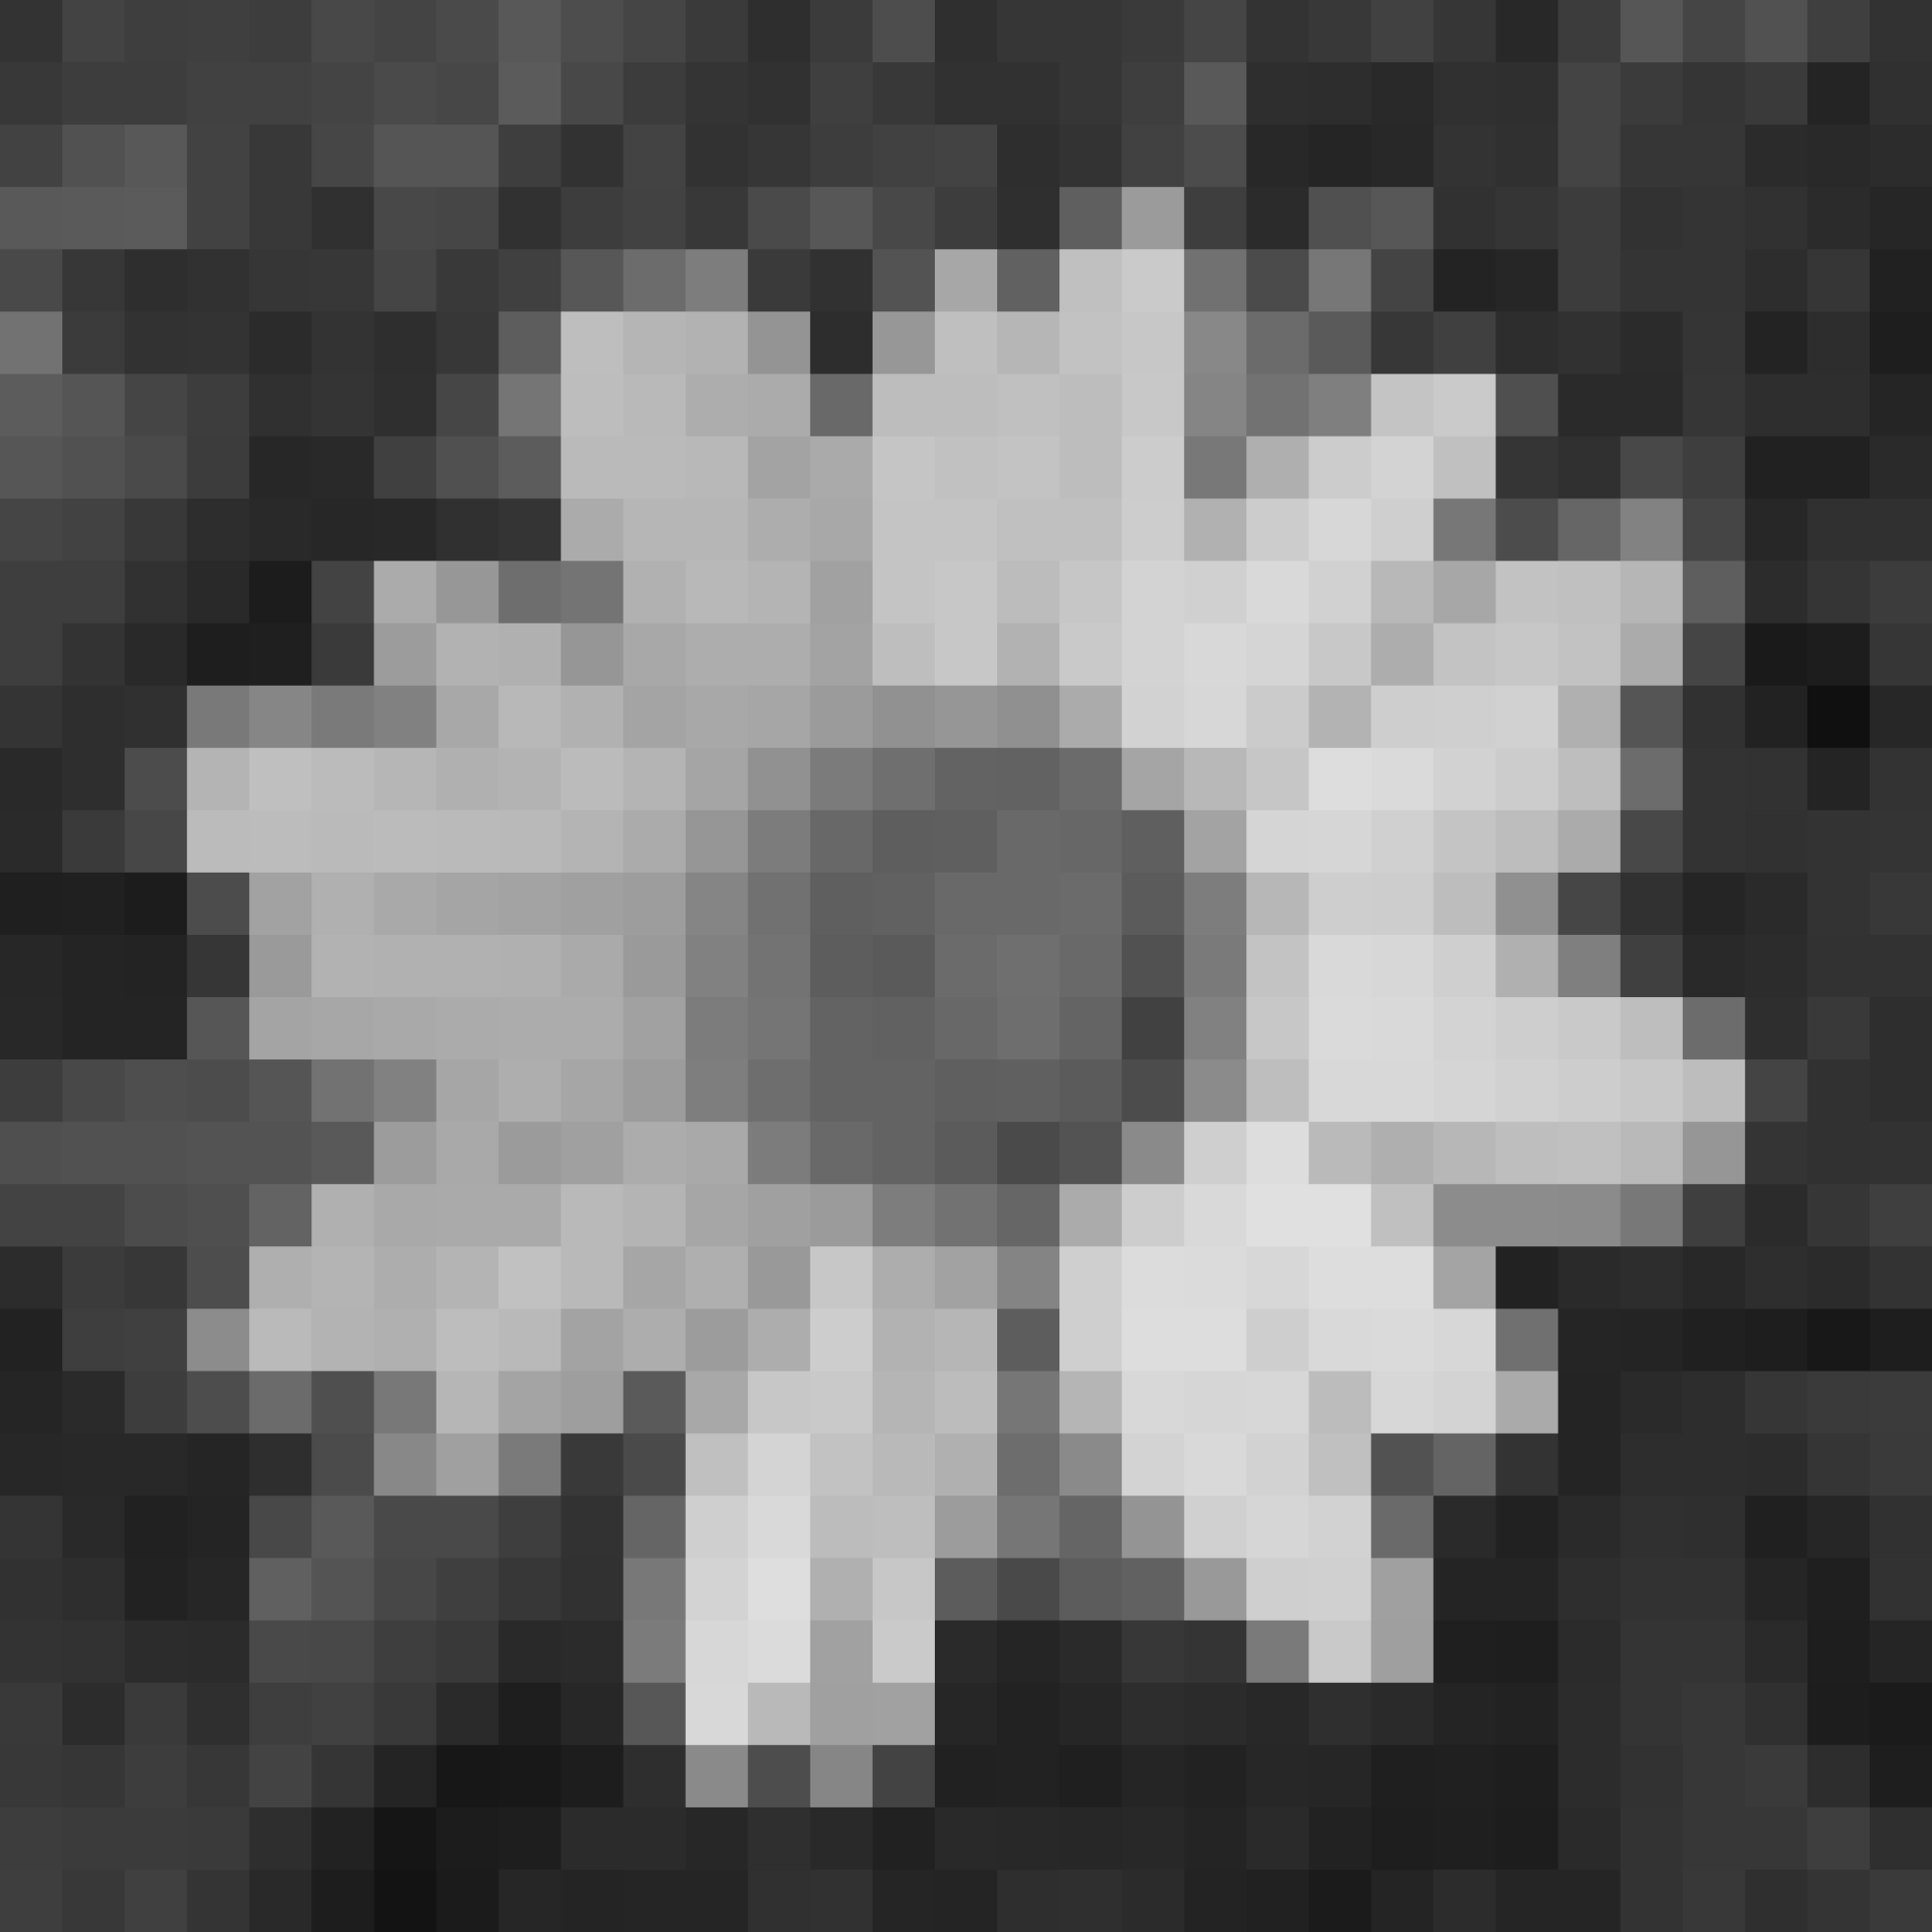
\includegraphics[interpolate=false, scale=0.09]{img/big_comp_fh} }}
    \caption{Comparación de imágenes}
    \label{fig:comp_fh}
\end{figure}

\section{Prueba completa}

A continuación mostramos el resultado del algoritmo de compresión al ser ejecutado sobre un set de 10 imágenes.

El promedio de compresión fue de aproximadamente 13\% y hemos tenido algunos casos en los cuales la imagen comprimida resultó ser de mayor tamaño que la original (aquellos en los que la compresión es negativa).

\begin{lstlisting}[language=bash]
make all
env/bin/python src/runner.py all
Running image:  source_images/01_mandril.png
Compression gain: 20.34 %
Running image:  source_images/02_lena.png
Compression gain: -4.34 %
Running image:  source_images/03_einstein.png
Compression gain: 17.31 %
Running image:  source_images/04_flower.png
Compression gain: 20.99 %
Running image:  source_images/05_loro.png
Compression gain: 14.45 %
Running image:  source_images/06_lena_face.png
Compression gain: -11.93 %
Running image:  source_images/07_puppy.png
Compression gain: 34.93 %
Running image:  source_images/08_random.png
Compression gain: -0.47 %
Running image:  source_images/09_picaflor.png
Compression gain: 20.61 %
Running image:  source_images/10_bebe.png
Compression gain: 1.17 %
\end{lstlisting}

\begin{figure}[!htbp]
    \centering
    \subfloat[01 mandril]{{ 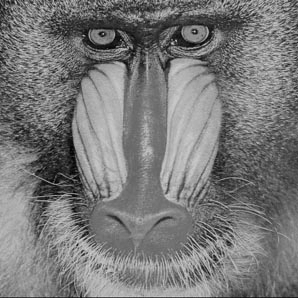
\includegraphics[interpolate=false, scale=0.4]{source_images/01_mandril} }}
    \qquad
    \subfloat[02 lena]{{ 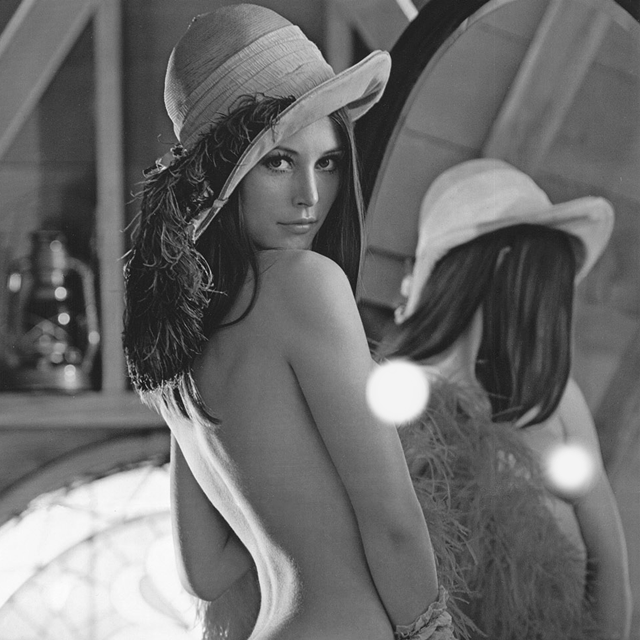
\includegraphics[interpolate=false, scale=0.2]{source_images/02_lena} }}
    \label{fig:all_img1}
\end{figure}

\begin{figure}[!htbp]
    \centering
    \subfloat[03 einstein]{{ 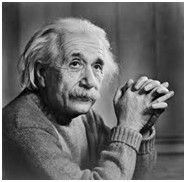
\includegraphics[interpolate=false, scale=0.6]{source_images/03_einstein} }}
    \qquad
    \subfloat[04 flower]{{ 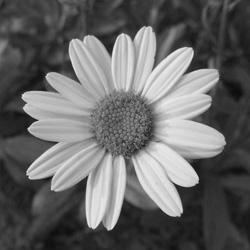
\includegraphics[interpolate=false, scale=0.4]{source_images/04_flower} }}
    \\
    \subfloat[05 loro]{{ 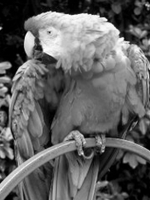
\includegraphics[interpolate=false, scale=0.6]{source_images/05_loro} }}
    \qquad
    \subfloat[06 lena face]{{ 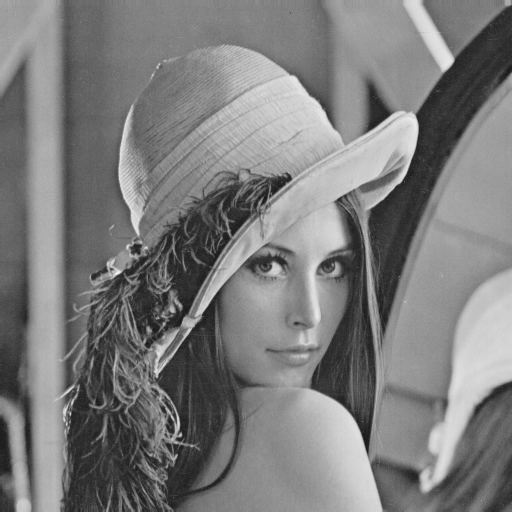
\includegraphics[interpolate=false, scale=0.2]{source_images/06_lena_face} }}
    \\
    \subfloat[07 puppy]{{ 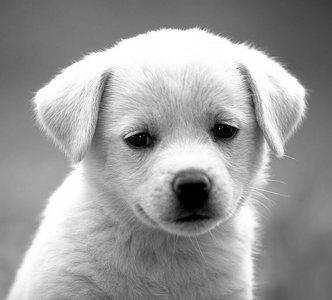
\includegraphics[interpolate=false, scale=0.4]{source_images/07_puppy} }}
    \qquad
    \subfloat[08 random]{{ 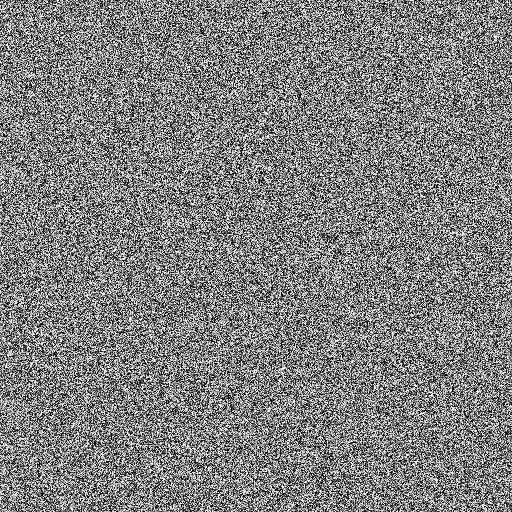
\includegraphics[interpolate=false, scale=0.2]{source_images/08_random} }}
    \\
    \subfloat[09 picaflor]{{ 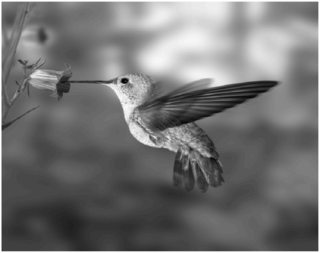
\includegraphics[interpolate=false, scale=0.4]{source_images/09_picaflor} }}
    \qquad
    \subfloat[10 bebe]{{ 
\includegraphics[interpolate=false, scale=0.2]{source_images/10_bebe} }}
    \label{fig:all_img2}
\end{figure}

\section{Observaciones}

\subsection{Limitaciones}
Descubrimos que debido a un problema con el algoritmo implementado, aquellas imágenes cuyas dimensiones no sean múltiplos de 8 contienen pérdida de información en la región izquierda e inferior.

A su vez, a la hora de querer recuperar una imagen codificada, descubrimos que nuestra implementación de la transformada inversa discreta del coseno es bastante lenta, tardando cerca de 20 segundos para recuperar la información de una imagen de aproximadamente 512x512 pixeles. 

\subsection{Lena}
\em{Lena} es una imagen que se utiliza recurrentemente en el análisis de algoritmos de procesamiento de imágenes\cite{wikipedia_Lena} debido a su detalle, sombreado, regiones de color planas y texturas.

Hemos descubierto que en ciertos casos (principalmente en fotos de Lena) el método de compresión genera imágenes de mayor peso que las originales, haciendo la compresión inefectiva. En la sección anterior podemos ver éste fenómeno.

\subsection{Mejoras}
Si bien codificamos la implementación original del algoritmo DCT, encontramos que existen variaciones sobre el algoritmo de la transformada discreta del coseno:

\subsubsection{Fast 2D-DCT}

Se puede implementar DCT en 2 dimensiones aplicando el algoritmo DCT a todas las filas de cada bloque y luego aplicar DCT a cada columna del bloque resultante. La complejidad de dicho algoritmo disminuye de $O(n^4)$ a $O(n^3)$\cite{unix4lyfe_DCT}.

\subsubsection{Algoritmo de Arai-Angui-Nakajima}

La idea es la misma que la del algoritmo anterior pero se reemplaza la implementación de la transformada discreta del coseno en 1 dimensión por una implementación similar a la transformada rápida de Fourier resultando en un algoritmo de complejidad $O(n\log{n})$. En nuestro trabajo, usamos ésta implementación para generar el reporte completo de compresiones ya que usando el original nos tomaba mucho tiempo. Para generar el reporte individual, usamos la implementación original\cite{unix4lyfe_AAN}\cite{unix4lyfe_DCT}.

\section{Conclusión}
Mediante el uso de la transformada de coseno y el algoritmo de codificación de Huffman hemos podido comprobar, dentro del conjunto de imágenes que conseguimos, que se puede comprimir (sin perdida de calidad) utilizando transformadas. La principal ventaja de utilizar DCT es que se "juntan" los datos de imagen de un bloque en un número casi óptimo de coeficientes descorrelacionados, dando lugar a una compresión significativa en algoritmos de codificacion aritmetica como Huffman.

La variacion que propusimos es aplicar un filtro, que si bien se pierde calidad en imagen final, luego de aplicar la antitransformada para conseguir la imagen original nuevamente, se gana una compresion que es inversamente proporcional al numero de frecuencias filtradas.

\section{Anexo}

\subsection{Como usar el codigo}
\subsubsection{Instalar}
\begin{lstlisting}[language=bash]
    git clone git@bitbucket.org:iLNaNo/mna-fft.git
    cd mna-fft
    make install
\end{lstlisting}
\subsubsection{Ejecutar}
\begin{lstlisting}[language=bash]
    make all
    make flower
    make ...
\end{lstlisting}

\subsection{Codigo Fuente}

\lstinputlisting[style=Style1, firstline=7, lastline=22, caption=DCT, label=code:dct]{src/dct_2.py}
\break
\lstinputlisting[style=Style1, firstline=21, lastline=53, caption=Funci\'{o}n complen, label=code:complen]{src/compress.py}
\lstinputlisting[style=Style1, firstline=7, lastline=18, caption=Huffman, label=code:huffman]{src/compress.py}
\break
\lstinputlisting[style=Style1, firstline=25, lastline=39, caption=DCT inversa, label=code:idct]{src/dct_2.py}
\lstinputlisting[style=Style1, firstline=42, lastline=46, caption=(I)DCT redondeado, label=code:quantize]{src/dct_2.py}


\printbibliography

\end{document}
